
\input{seadistus.tex}

% Meta-andmed
\title{Suurte keelemudelite kasutamine eestikeelse tehnilise informaatika teksti kvaliteedikontrolliks}
\author{Uku Renek Kronbergs}
\date{2026}
\supervisor{Alo Peets\degree{MSc}}
\curriculum{Informaatika õppekava}
\thesis{Bakalaureusetöö (9 EAP)}
\keywords{Suured keelemudelid, eesti keel, akadeemiline tekst, tagasiside, kvaliteedikontroll, promptimine}


% Siit algab dokument

\begin{document}

\maketitle

\linespread{1.45} \selectfont

\newpage
\pdfbookmark[1]{\infoname}{info} % Lisame infolehe PDF-faili järjehoidjatesse.

% Eesti keeles info.
\begin{info}
\begin{abstract}
Eestikeelse informaatika lõputöö kirjutamine on tudengile keeleliselt ja struktuurselt nõudlik ülesanne, sest valdkonna terminoloogia on inglise keeles välja kujunenud ning akadeemilise stiili reegleid kohaldatakse eesti keeles erinevalt. Käesoleva bakalaureusetöö eesmärk on luua ja hinnata suurel keelemudelil põhinev prototüüp, mis annab eestikeelsele informaatika lõputöö tekstile automaatset tagasisidet neljas kategoorias: struktuur, akadeemiline stiil, terminoloogia järjepidevus ja viitamisvajadus. Töös käsitletakse suurte keelemudelite võimekust eestikeelse tehnilise teksti analüüsimisel ning struktureeritud promptimise mõju tagasiside kvaliteedile. Prototüüp on realiseeritud veebirakendusena, mis võtab sisendiks tudengi kirjutatud peatüki, suunab selle valitud keelemudelile struktureeritud viibaga ning kuvab kasutajale kategoriseeritud tagasiside. Süsteemi hindamiseks koostati 20 tekstikatkendist koosnev testkogu, milles probleemid märgendati käsitsi koos juhendajaga. Mudeli väljundit võrreldi kuldstandardiga täpsuse, saagise ja F\textsubscript{1}-skoori abil. Tulemused näitavad, et struktureeritud promptimine annab kõikides kategooriates üldisest viibast täpsemat tagasisidet, kusjuures mudel on kõige usaldusväärsem viitamisvajaduse ja struktuuri tuvastamisel ning kõige problemaatilisem terminoloogia järjepidevuse hindamisel. Töös rõhutatakse, et süsteem on tudengi enda kirjutatud teksti tagasisidevahend, mitte juhendaja ega tekstigeneraator.
\end{abstract}

\keywords{}

\cercs{P175 Informaatika, süsteemiteooria}
% Koodid leiate: https://www.etis.ee/Portal/Classifiers/Index/26
\end{info}


% Inglise keeles info.
\begin{otherInfo}{english}{Using Large Language Models for Quality Control of Estonian Technical Computer Science Texts}
\begin{abstract}
Writing a computer science thesis in Estonian is linguistically and structurally demanding for a student because the field's terminology has evolved in English and academic style conventions are applied differently in Estonian. The aim of this bachelor's thesis is to design and evaluate a prototype based on a large language model (LLM) that provides automatic feedback on Estonian-language computer science thesis texts in four categories: structure, academic style, terminological consistency, and the need for citation. The thesis examines the capability of large language models to analyse Estonian technical text and the effect of structured prompting on the quality of the resulting feedback. The prototype is implemented as a web application that takes a student-written chapter as input, sends it to the chosen language model with a structured prompt, and presents categorised feedback to the user. To evaluate the system, a test set of 20 text excerpts was created, with issues annotated manually together with the supervisor. The model's output was compared against this gold standard using precision, recall, and F\textsubscript{1}-score. The results indicate that structured prompting yields more accurate feedback than a generic prompt across all categories, that the model is most reliable when detecting the need for citation and structural problems, and least reliable when assessing terminological consistency. The thesis emphasises that the system is a feedback tool for text the student has written themselves; it neither replaces the supervisor nor generates the thesis on the student's behalf.
\end{abstract}

\keywords{Large language models, Estonian language, academic text, feedback, quality control, prompting}

\cercs{P175 Informatics, systems theory}
\end{otherInfo}


\tableofcontents

\section{Sissejuhatus} \label{sissejuhatus}

Bakalaureusetöö kirjutamine on iga informaatika tudengi õpingute lõpus tehtav mahukas iseseisev töö, mille puhul hinnatakse nii teaduslikku panust kui ka töö vormistamist ja keelelist kvaliteeti. Tartu Ülikooli arvutiteaduse instituudi nõuetes moodustab vormistamine ligi 25~\% lõputöö koondhindest~\cite{ut_juhend_2024}, kusjuures suurt rõhku pannakse selgele struktuurile, akadeemilisele stiilile, terminoloogia järjepidevusele ja korrektsele viitamisele. Eestikeelses informaatika lõputöös on neid nõudeid eriti keeruline täita, sest valdkonna terminoloogia on suuresti arenenud välja inglise keeles ning paljudele mõistetele puudub väljakujunenud eestikeelne vaste või on neid mitu.

Suurte keelemudelite (\emph{ingl.\ large language model}, edaspidi LLM) viimaste aastate areng on toonud kaasa loomuliku keele töötluse vahendid, mis suudavad analüüsida ja parandada mahukaid tekste märkimisväärse usaldusväärsusega~\cite{brown_language_2020, openai_gpt4_2023, anthropic_claude_2024}. Kui veel mõni aasta tagasi olid sellised vahendid valdavalt ingliskeelsed, siis tänapäevased mitmekeelsed mudelid, nagu Claude 4.7 Opus, GPT-5.5 ja Gemini 2.x, suudavad mõistliku kvaliteediga töödelda ka eesti keelt, mida kinnitavad TartuNLP avalikud võrdlused (vt baromeeter~\cite{tartunlp_baromeeter_2025}). See loob võimaluse rakendada LLM-e tudengite toetamiseks erialadel, kus eestikeelne akadeemiline kirjutamine on traditsiooniliselt olnud keeruline.

Akadeemilises kontekstis on LLM-ide kasutamine samas eetiliselt tundlik teema. Tartu Ülikooli generatiivse tehisaru kasutamise juhend~\cite{ut_genAI_2024} eristab selgelt teksti \emph{loomist} (mis ei ole lõputöös tudengi enda panusena lubatud) ja teksti \emph{tagasisidestamist} (mis on lubatud, kui tudeng saadud soovitusi ise kriitiliselt hindab ja rakendab). Käesolevas töös käsitletav süsteem kuulub üheselt teise kategooriasse: see ei kirjuta lõputööd tudengi eest ega asenda juhendajat, vaid annab tudengi enda kirjutatud tekstile soovituslikku tagasisidet. See eristus on teema akadeemilise vastuvõetavuse jaoks kriitilise tähtsusega ning seda tuleb selgelt rõhutada nii süsteemi kasutajaliideses kui ka tagasiside tekstis endas.

\subsection*{Töö eesmärk ja ulatus}

Käesoleva bakalaureusetöö \textbf{eesmärk} on \emph{kavandada ja realiseerida} LLM-il põhinev prototüüp, mis annab eestikeelsele informaatika lõputöö tekstile automaatset tagasisidet struktuuri, akadeemilise stiili, terminoloogia järjepidevuse ja viitamisvajaduse kohta, ning \emph{hinnata} selle väljundi kvaliteeti nii kvalitatiivse pilootuuringu kui ka sünteetilisel testkogul tehtud empiirilise hindamisega.

\textbf{Töö ulatus.} Käesoleva töö raames tehti:
\begin{enumerate}
    \item tagasisidekategooriate operatsionaalne määratlus;
    \item kahe promptimisstrateegia (üldine ja struktureeritud) disain;
    \item veebipõhise prototüübi realiseerimine, sealhulgas demo-režiim, mis võimaldab süsteemi proovida ilma välise LLM-i API juurdepääsuta;
    \item kvalitatiivne pilootuuring väikesel tekstivalimil prompti disaini iteratsiooniks ja mudeli väljundi tüüpiliste mustrite tuvastamiseks;
    \item 20-katkendilise sünteetilise testkogu ja kuldstandardi koostamine (autori juhendamisel LLM-iga; vt allpool generatiivse tehisaru deklaratsioon);
    \item täismahuline empiiriline hindamine 80 päris API-päringu põhjal (kaks mudelit × kaks prompti × 20 katkendit) koos täpsuse, saagise ja F\textsubscript{1}-skoori arvutamisega iga (mudel × promptitüüp × kategooria) kombinatsiooni kohta.
\end{enumerate}

\textbf{Töö ulatusest on teadlikult välja jäetud}: päris üliõpilastöödel põhinev testkogu (käesolev testkogu on sünteetiline) ning sõltumatu teise annoteerija kaasamine kuldstandardi koostamisse (käesoleva töö kuldstandard on ühe annoteerija ehk autori koostatud). Nende sammude jätkukava on esitatud peatükis~\ref{hindamine:edasine}. Selline ulatusepiirang on motiveeritud sellega, et päris üliõpilastööde põhjal kuldstandardi koostamine koos sõltumatu teise annoteerijaga nõuab eraldi tööd, mis kuulub edasisse uurimisse (näiteks magistriõppes või avaldatavas artiklis).

\subsection*{Uurimisküsimused}

Käesolev töö käsitleb järgmisi \textbf{uurimisküsimusi}, millele antakse vastused nii kvalitatiivse pilootuuringu (peatükk~\ref{hindamine:arutelu}) kui ka sünteetilisel testkogul tehtud kvantitatiivse empiirilise hindamise põhjal (peatükk~\ref{hindamine:synteetiline}); sama metoodika kohaldamine päris üliõpilastöödele kuulub jätkukavasse (peatükk~\ref{hindamine:edasine}):
\begin{enumerate}
    \item Millise iseloomuga tagasisidet annab tippkvaliteediga LLM eestikeelse informaatika lõputöö tekstile, kui talle antakse struktureeritud kategoorianõuetega prompt?
    \item Millistes tagasisidekategooriates on mudeli väljund kõige usaldusväärsem ning millistes kõige problemaatilisem, ja miks?
    \item Kas struktureeritud promptimine annab üldisest promptist süsteemsemat ja kasutuskõlblikumat tagasisidet?
\end{enumerate}

Töö keskne \textbf{hüpotees} -- mida uurimisküsimus~3 operatsionaliseerib -- on, et struktureeritud kategooria- ja skeemipõhine promptimine annab eestikeelse informaatika lõputöö tekstile tagasiside andmisel üldisest viibast süsteemsemat ja kasutuskõlblikumat väljundit (vt täpsem sõnastus peatükis~\ref{taust:promptimine}).

Pilootuuringu tähelepanekud ja empiirilised tulemused, mis nendele küsimustele vastavad, on esitatud peatükis~\ref{hindamine}.

\subsection*{Praktiline panus ja piirangud}

Töö praktiline tulemus on lokaalselt käivitatav veebiprototüüp, kus kasutaja saab valida lõputöö peatükitüübi (sissejuhatus, taust, metoodika, tulemused, kokkuvõte), sisestada enda kirjutatud teksti ning saada struktureeritud tagasisidet neljas eelnimetatud kategoorias. Prototüüp on kavandatud nii, et seda saab proovida \emph{demo-režiimis} salvestatud näidisvastustega ilma välise LLM-i API juurdepääsuta, mis muudab töö praktilise tulemuse reprodutseeritavaks minimaalsete eeldustega.

\textbf{Töö ei käsitle} LLM-i kasutamist lõputöö \emph{loomiseks}. Süsteem on mõeldud tudengi enda kirjutatud tekstile tagasiside saamiseks ega püüa asendada juhendaja sisulist tagasisidet. Mudeli soovitused on kasutaja jaoks vaid lähtepunkt -- iga soovituse vastuvõtmine, ümbersõnastamine või tagasilükkamine on tudengi enda otsustada.

\subsection*{Töö ülesehitus}

Peatükis~\ref{taust} esitatakse ülevaade suurte keelemudelite arhitektuurist, eestikeelsest LLM-tugist ja akadeemilise teksti automaatsest tagasisidestamisest, samuti kirjeldatakse seotud töid. Peatükk~\ref{metoodika} määratleb tagasisidekategooriad ning kirjeldab prompti disaini põhimõtteid ja hindamismetoodikat. Peatükis~\ref{prototuup} kirjeldatakse prototüübi arhitektuuri, tehnoloogilist lahendust ja kasutajaliidese disaini. Peatükk~\ref{hindamine} esitab pilootuuringu kvalitatiivsed tähelepanekud, sünteetilisel testkogul tehtud empiirilise hindamise tulemused ning päris üliõpilastöödel põhineva jätkuhindamise kava. Peatükis~\ref{kokkuvõte} antakse kokkuvõte töö panusest ning visandatakse võimalused edasiseks uurimiseks. Lisas~I on esitatud kasutatud sünteetilise testkogu kirjeldus ja kavandatud päris testkogu disain, lisas~II struktureeritud prompti täielik tekst, lisas~III lähtekoodi ja andmestiku struktuur ning lisas~IV prototüübi kasutusjuhend (sealhulgas demo-režiimi käivitamine ilma API-võtmeta).

\subsection*{Generatiivse tehisaru kasutamise deklaratsioon}

Käesoleva töö koostamisel on generatiivset tehisaru (peamiselt Anthropici mudelit Claude 4.7 Opus) kasutatud järgmisel kolmel viisil, mille autor selgesõnaliselt deklareerib:

\begin{enumerate}
    \item \textbf{Tekstilise abivahendina} -- loetavuse parandamiseks, sõnastuse poleerimiseks ja struktuurinõustamiseks. Kõik sisulised mõtted, töö ulatuse valikud, metoodilised valikud ja järeldused on autori enda otsused. Mudeli ettepanekud vaadati iga kord kriitiliselt üle ning sõnastati vajaduse korral ümber või jäeti kõrvale.
    \item \textbf{Hindamise testkogu ja kuldstandardi koostamise abivahendina} -- alapeatükis~\ref{hindamine:synteetiline} esitatud empiirilise hindamise jaoks on 20 testkatkendit (igaüks ligikaudu 100--160 sõna) ja 42 kuldstandardi annotatsiooni koostatud autori juhendamisel mudeliga Claude 4.7 Opus \emph{interaktiivse vestlusliidese kaudu (Claude Code)}, mitte programmiliste API-päringute kaudu. See ühekordne genereerimisprotsess on metoodiliselt eraldatud alapeatükis~\ref{hindamine:synteetiline} kirjeldatud hindamispäringutest, mis kasutavad Anthropici ja OpenAI tasulisi API-sid skriptipõhiselt; testkogu ja kuldstandardi koostamine ei toimunud nende API-de kaudu. Tegu ei ole anonüümitud üliõpilastööde katkenditega, vaid sünteetiliste tekstidega, mis on koostatud nii, et katkendid sisaldaksid ette nähtud tüüpilisi probleeme tagasisidekategooriates. See piirang on selgesõnaliselt välja toodud alapeatükis~\ref{hindamine:synteetiline} ning piirangute jaotises~\ref{hindamine:piirangud}. Päris üliõpilastööde katkendite kasutamine kuulub jätkukavasse (vt alapeatükk~\ref{hindamine:edasine}).
    \item \textbf{Hinnatavate mudelivastuste tegelike API-päringute kaudu} -- alapeatükis~\ref{hindamine:synteetiline} esitatud F\textsubscript{1}-skoorid \emph{on tegelikud empiirilised mõõtmised}: iga (katkend × promptitüüp × mudel) kombinatsiooni jaoks tehti tegelik API-päring Anthropici mudelile Claude 4.7 Opus või OpenAI mudelile GPT-5.5 (kokku 80 päringut), salvestati toorvastus repositooriumi kausta \texttt{statistika/andmed/paris\_vastused/} ning skooriti tekstivahemiku tasemel kattuvuse järgi kuldstandardi vastu. \emph{Need numbrid kajastavad tegelikku mudelite sooritust} antud sünteetilisel testkogul, kuid nende üldistatavus päris üliõpilastöödele on piiratud, kuna testkogu ise on sünteetiline (vt punkt 2).
\end{enumerate}

Selline kasutus on otseses kooskõlas Tartu Ülikooli generatiivse tehisaru juhendiga~\cite{ut_genAI_2024}, mis lubab generatiivse tehisaru kasutamist õppetöös \emph{tingimusel, et selline kasutus on selgesõnaliselt deklareeritud}. Reprodutseerimiseks vajalikud skriptid, salvestatud API-vastused ja andmestik on saadaval töö repositooriumis (\url{https://github.com/UkuRenekKronbergs/TI_bakalaureusetoo}) kaustas \texttt{statistika/}. Lugeja saab seal kontrollida, kuidas iga arv on saadud (failid \texttt{andmestik\_synth.py}, \texttt{paris\_hindamine.py} ning vastuste JSON-id alamkaustas \texttt{paris\_vastused/}).

\section{Taust ja seotud tööd} \label{taust}

Käesolevas peatükis antakse ülevaade töö tausta moodustavatest valdkondadest. Alapeatükis~\ref{taust:llm} kirjeldatakse suurte keelemudelite arhitektuurset alust ja võimekust. Alapeatükk~\ref{taust:eesti} käsitleb LLM-ide võimekust eesti keeles ning sellega seotud kitsaskohti. Alapeatükis~\ref{taust:akadeemiline} määratletakse akadeemilise teksti kvaliteediomadused, millele süsteem tagasisidet annab. Alapeatükk~\ref{taust:promptimine} esitab promptimise põhimõtted, mis on prototüübi disainile aluseks. Lõpuks vaadeldakse alapeatükis~\ref{taust:seotud} teksti tagasisidestamise olemasolevaid lahendusi ja akadeemilist kirjandust.

\subsection{Suured keelemudelid} \label{taust:llm}

Suur keelemudel on isejuhendatud õppega närvivõrk, mis on treenitud väga suurel loomuliku keele andmestikul nii, et ta suudab etteantud tekstiosa põhjal ennustada järgnevat sõna~\cite{vaswani_attention_2017, brown_language_2020}. Tänapäevased mudelid põhinevad \emph{Transformer}-arhitektuuril~\cite{vaswani_attention_2017}, milles keskne mehhanism on enesetähelepanu (\emph{ingl.\ self-attention}). See mehhanism võimaldab mudelil iga sõna esituses arvesse võtta kõigi eelnevate (ning mõnel juhul ka järgnevate) sõnade konteksti, mis teeb mudeli pikkade sõltuvuste tuvastamisel oluliselt võimekamaks kui varem domineerinud rekurrentsed närvivõrgud~\cite{hochreiter_lstm_1997}.

Mudeli treenimine jaguneb tüüpiliselt kaheks etapiks: eelkoolitus (\emph{ingl.\ pre-training}) suurtel struktureerimata tekstikorpustel ning järelhäälestus (\emph{ingl.\ fine-tuning}) konkreetseteks ülesanneteks. Juhiseid järgivate mudelite (nagu GPT, Claude, Gemini) puhul lisandub veel inimtagasiside abil õppimine (\emph{ingl.\ reinforcement learning from human feedback}, RLHF)~\cite{ouyang_instructgpt_2022}, mille käigus mudel kohandatakse vastama loomuliku keele juhistele turvaliselt ja kasulikult.

Treeningu mahukus on väga kiiresti kasvanud. Nii GPT-3 (175 miljardit parameetrit, 2020)~\cite{brown_language_2020} kui ka selle järglased on näidanud nähtust, mida on hakatud nimetama \emph{esiletõusvateks võimeteks} (\emph{ingl.\ emergent abilities}): mudelid lahendavad ülesandeid, mille jaoks neid spetsiaalselt ei treenitud, kui parameetrite arv ja andmemaht ületavad teatud piiri~\cite{wei_emergent_2022}. Just see omadus võimaldab kasutada üht ja sama mudelit nii teksti kokkuvõtmiseks, küsimustele vastamiseks kui ka käesolevas töös käsitletud tagasiside andmiseks.

LLM-ide kasutamisega kaasnevad ka tuntud puudujäägid. Mudelid võivad esitada faktiliselt ekslikke väiteid suure enesekindlusega (\emph{ingl.\ hallucination})~\cite{ji_hallucination_2023}, mille olulisust akadeemilise teksti kontekstis ei saa alahinnata. Lisaks võivad mudelid jäljendada treeningandmetes esinevaid süstemaatilisi kallutusi ning ühe konkreetse mudeli väljund ei pruugi olla deterministlik: sama prompt võib eri kordadel anda erinevaid tulemusi.

\subsection{LLM-id eesti keeles} \label{taust:eesti}

Eesti keel on inglise keelega võrreldes vähese ressursiga keel: kuigi tegu ei ole maailma kõige väiksema kõnelejaskonnaga keelega, on eestikeelse digitaalse teksti maht oluliselt väiksem ning seetõttu on eesti keele esindatus tüüpilises mitmekeelses treeningkorpuses (näiteks Common Crawl) väga tagasihoidlik. Sellele vaatamata on viimaste põlvkondade üldotstarbelistes mudelites eesti keele kvaliteet märgatavalt paranenud. Tartu Ülikooli loomuliku keele töötluse uurimisrühma (TartuNLP) avalik eesti keele LLM-võrdlusplatvorm (baromeeter)~\cite{tartunlp_baromeeter_2025} võrdleb nii avatud kui ka kommertsiaalsete mudelite jõudlust eestikeelsetel ülesannetel ning näitab, et tipptasemel mitmekeelsed mudelid (sh Claude 4.x ja GPT-5.5) kuuluvad eesti keele kvaliteedi poolest tippu, kuigi jäävad üldjuhul alla võrreldavale inglise keele tasemele.

Lisaks üldotstarbelistele LLM-idele on Eestis arendatud spetsiaalseid eesti keele mudeleid. EstBERT~\cite{tanvir_estbert_2021} on BERT-arhitektuuril põhinev mudel, mis on eelkoolitatud eestikeelsel korpusel ning sobib selliste klassifitseerimisülesannete jaoks nagu sentiment- ja teemaanalüüs. EstBERT-i kasutamine teksti genereerimist nõudvate ülesannete jaoks on aga piiratud, kuna mudel on arhitektuurselt enkooderitüüpi. Eestikeelseid generatiivseid mudeleid on hakatud aktiivselt arendama hiljutiste avatud lähtekoodiga mudelite (näiteks Llama-2 ja Llama-3) baasil -- nii on TartuNLP koostanud Llammas-mudeli, mille treenimine ja hindamine on dokumenteeritud Kuulmetsa jt töödes~\cite{kuulmets_llammas_2024, kuulmets_finnougri_2025} --, kuid nende ulatus jääb tippkommertsmudelite omale alla.

Praktilises rakenduses tähendab see, et eestikeelse akadeemilise teksti analüüsiks on otstarbekam kasutada tippkvaliteediga mitmekeelseid mudeleid (Claude 4.7 Opus, GPT-5.5) kui spetsialiseeritud avatud mudeleid, kui prioriteediks on kvaliteet, mitte kohaliku andmetöötluse nõue.

\subsection{Akadeemilise teksti kvaliteediomadused} \label{taust:akadeemiline}

Akadeemilise teksti kvaliteet on mitmemõõtmeline. Burstein jt~\cite{burstein_aes_2013} on automaatse esseede hindamise (\emph{ingl.\ automated essay scoring}, AES) ülevaates eristanud vähemalt järgmisi mõõtmeid: sisuline asjakohasus, organiseeritus, sõnavara, stiili sobivus ning õigekirja- ja vormistusvead. Käesolevas töös on rõhk neljal omadusel, mis on Tartu Ülikooli arvutiteaduse instituudi nõuete~\cite{ut_juhend_2024} kontekstis kõige otsesemalt hinnatavad ja mille puhul automaatne tagasiside on praktilise väärtusega.

\subsubsection{Struktuur}

Lõputöö struktuur peab olema lugejale loogiliselt järgitav. Iga peatükk algab sissejuhatava lõiguga, alampeatükid peavad olema teemaga seotud, peatüki sees on hea kasutada siduvaid lauseid eri lõikude vahel ning peatüki lõpus võiks olla sünteesilõik. Peatükk ei peaks algama ega lõppema joonise, tabeli ega loeteluga ilma teksti vaheta~\cite{ut_juhend_2024}. Strukturaalsed probleemid hõlmavad seega liiga lühikesi peatükke, sissejuhatava lõigu puudumist, ebaloogilist alampeatükkide järjekorda ja sujumatut lõikudevahelist üleminekut.

\subsubsection{Akadeemiline stiil}

Akadeemiline stiil eestikeelses lõputöös järgib eesti keele head tava ja teadusliku kirjutamise norme. Tüüpilised stiilivead on järgmised: kõnekeelsete väljendite kasutamine (näiteks \emph{tüüp}, \emph{asi}, \emph{teha}); umbisikuline tegumood seal, kus seda ei nõuta, või vastupidine viga; mina-vormi liigne kasutamine; liiga pikad ja keerulised laused; kvalifitseerimata üldistused (\emph{kõik teavad, et\dots}); inglise keele otsetõlke ilmingud (näiteks \emph{see on tõsi, et\dots} kui konstruktsiooni \emph{it is true that\dots} otsetõlge). Hyland~\cite{hyland_metadiscourse_2005} on rõhutanud, et akadeemiline stiil ei ole pelgalt sõnavara valik, vaid ka selge metadiskursus, mis juhib lugejat läbi teksti.

\subsubsection{Terminoloogia järjepidevus}

Tehnilises informaatikatekstis on terminoloogiavalik eriti oluline. Sama mõiste kohta tuleks kasutada läbivalt sama terminit (näiteks \emph{andmebaas}, mitte vaheldumisi \emph{andmebaas} ja \emph{baas}; või \emph{lõim}, mitte vaheldumisi \emph{lõim} ja \emph{niit}). Tihti tuleb teha valik kahe võrdselt levinud variandi vahel, näiteks \emph{kasutaja\-liides} ja \emph{kasutaja\-pind}, \emph{järjend} ja \emph{loend}, \emph{kompileerimine} ja \emph{tõlkimine}. Eesti Keele Instituudi terminisõnastik\footnote{\url{https://termin.eki.ee/}} ja Tartu Ülikooli arvutiteaduse instituudi sõnastikud annavad osa juhiseid, kuid sageli peab autor tegema iseseisva valiku ning seda järjekindlalt rakendama. Lisaks kerkib küsimus, millal tuua sisse ingliskeelne termin (\emph{kursiivis sulgudes}) ja millal seda enam mitte korrata.

\subsubsection{Viitamisvajadus}

Iga väide, mis ei ole autori enda originaalne mõte ega üldteadmine, vajab viidet allikale. Vastasel juhul on tegu akadeemilise petturlusega. Levinud probleemid on järgmised: viiteta esitatud arvulised väited (\emph{75~\% kasutajatest eelistab\dots}); konkreetne metoodika või algoritm, mille puhul viidet pole esitatud; teiste autorite definitsioonide refereerimine ilma viiteta. LLM-i ülesanne ei ole \emph{ise} viiteid leida, vaid anda märku, kus viide on tõenäoliselt vajalik; lõplik otsus ja kontroll jäävad autorile.

\subsection{Promptimine ja struktureeritud viibad} \label{taust:promptimine}

LLM-i käitumist juhitakse \emph{prompti} ehk viiba abil – see on tekstiline juhis, mille mudel saab koos analüüsitava sisendiga. Viiba kvaliteet mõjutab mudeli väljundit oluliselt. Promptimisstrateegiate ülevaates~\cite{liu_prompting_2023} eristatakse muu hulgas:

\begin{itemize}
    \item \textbf{Nullhetk-promptimine} (\emph{ingl.\ zero-shot prompting}) – mudelile antakse ainult ülesanne ja sisend, näideteta.
    \item \textbf{Vähehetk-promptimine} (\emph{ingl.\ few-shot prompting}) – ülesandele lisatakse mõned näited oodatava sisendi-väljundi paari kohta.
    \item \textbf{Mõtteahel-promptimine} (\emph{ingl.\ chain-of-thought prompting}) – mudelilt küsitakse selgesõnaliselt vahesammude põhjendust enne lõplikku vastust~\cite{wei_chain_2022}.
    \item \textbf{Struktureeritud väljundi nõue} – mudelilt nõutakse väljundit kindlal kujul, näiteks JSON-i, mis lihtsustab automaatset järeltöötlust~\cite{geng_structured_2025}.
\end{itemize}

Käesolevas töös testitakse kaht promptimisstrateegiat. Mõlemad nõuavad mudelilt sama JSON-skeemiga väljundit, et automaatne järeltöötlus oleks võrreldav. \emph{Üldine} (\emph{baseline}) prompt esitab mudelile vaid rolli ja minimaalse JSON-skeemi (lisaks neljale tagasisidekategooriale lubatud ka \texttt{MUU}), kuid \emph{ei sisalda} kategooriate definitsioone, näiteid ega täpsustavaid reegleid. \emph{Struktureeritud} prompt määrab täpselt neli kategooriat, esitab iga kategooria kohta näiteid ja vastunäiteid, sisaldab mõtteahela elementi (mudel peab iga tuvastatud probleemi jaoks põhjendama, miks ta seda probleemiks peab) ning sõnastab konservatiivsusele suunavaid reegleid. Hüpotees on, et struktureeritud prompt annab täpsemat ja võrreldavamat väljundit.

\subsection{Seotud tööd} \label{taust:seotud}

Automaatse teksti tagasisidestamise valdkonnal on pikk ajalugu. Klassikalised süsteemid, nagu Criterion~\cite{burstein_criterion_2004} ja e-rater~\cite{attali_erater_2006}, on alates 2000. aastatest võimaldanud esseetasemel tagasisidet, kuid on välja töötatud peamiselt inglise keele jaoks. Grammarly~\cite{grammarly_2024} on tänapäeval üks enim kasutatud kommertsiaalseid stiili- ja grammatikakontrolli vahendeid, mille eesti keele tugi on 2026.~aasta seisuga endiselt piiratud.

Teadusartiklite kvaliteedi automaatset tagasisidestamist on uuritud süsteemides, nagu SciScore~\cite{menke_sciscore_2020} ja Paper Robot~\cite{wang_paperrobot_2019}, kuid need keskenduvad metoodika reprodutseeritavusele ja struktureeritud kontrollnimekirjadele, mitte üldisele stiilile ja terminoloogiale. LLM-ide tulekuga on hakanud ilmuma tööd, mis kasutavad GPT-4 ja Claude'i akadeemiliste kirjutiste tagasisidestamiseks~\cite{liang_chatgpt_2024, kasneci_chatgpt_2023}. Liang jt~\cite{liang_chatgpt_2024} näitavad, et GPT-4 teadusartiklitele antud tagasiside kattub umbes 30--39~\% ulatuses inimretsensentide tagasisidega; see protsent on madalam kui inimretsensentide omavaheline kattuvus, kuid sellele lähedane.

Eestikeelse akadeemilise teksti automaatset tagasisidestamist on uuritud oluliselt vähem. Käesoleva töö raames ei õnnestunud tuvastada avaldatud uurimusi, mis käsitleksid spetsiaalselt eestikeelsete informaatika lõputööde automaatset tagasisidestamist generatiivsete LLM-ide abil. Käesolev töö täidab seda lünka kahel viisil: esiteks rakendab süsteemi spetsiaalselt informaatika lõputöödele, kus tehniline terminoloogia mängib suurt rolli, ja teiseks kasutab generatiivseid LLM-e koos struktureeritud promptiga.

Promptimise mõju kvaliteedile on samuti uuritud. Schulhoff jt~\cite{schulhoff_prompt_report_2024} on promptimistehnikaid süstemaatiliselt katalogiseerinud ning näitavad, et struktureeritud promptid annavad spetsiifilistel ülesannetel tüüpiliselt suuremat täpsust. Käesolev töö rakendab seda eestikeelse akadeemilise teksti analüüsile.

Käesoleva töö \textbf{teaduslik panus} on seega: (1) struktureeritud LLM-prompti disain eestikeelse informaatikateksti tagasisidestamiseks neljas kategoorias, (2) 20-katkendilise sünteetilise testkogu ja kuldstandardi koostamine koos hindamismetoodikaga ning (3) üldise ja struktureeritud prompti empiiriline võrdlus kahe tippmudeli põhjal, mille tulemused näitavad struktureeritud prompti järjepidevat eelist.

\section{Metoodika} \label{metoodika}

Käesolev peatükk kirjeldab, kuidas töö eesmärki realiseeritakse. Alapeatükis~\ref{metoodika:protsess} esitatakse uurimisprotsess tervikuna ning eristatakse selgelt, millised sammud on käesoleva töö raames lõpule viidud ja millised on kavandatud jätkukavasse. Alapeatükk~\ref{metoodika:kategooriad} määratleb tagasisidekategooriad operatsionaalselt. Alapeatükis~\ref{metoodika:mudel} põhjendatakse mudeli valikut. Alapeatükk~\ref{metoodika:promptid} esitab kahe võrreldava prompti disaini. Alapeatükis~\ref{metoodika:hindamine} kirjeldatakse \emph{kavandatud} täismahulise hindamise metoodikat ja testkogu disaini.

\subsection{Uurimisprotsess} \label{metoodika:protsess}

Uurimine järgib disain\-teaduse (\emph{ingl. design science research}) põhimõtet~\cite{hevner_design_2004}: identifitseeritakse probleem, projekteeritakse artefakt (käesoleval juhul prototüüp), rakendatakse seda ning hinnatakse rangelt. Hindamise põhjal saab teha järeldusi nii artefakti kui ka selle aluseks olevate disainivalikute kohta.

Töö protsess on kavandatud koosnema järgmistest etappidest:
\begin{enumerate}
    \item Tagasisidekategooriate operatsionaalne määratlemine kirjanduse ja TÜ juhendi põhjal.
    \item Üldise ja struktureeritud prompti disain.
    \item Prototüübi realiseerimine veebirakendusena, mis kutsub välja LLM-i API-d ning toetab salvestatud vastustega demo-režiimi.
    \item Testkogu disain: 20 eestikeelset informaatika lõputöö katkendit erinevatest peatükitüüpidest, koos kuldstandardi koostamise protseduuriga.
    \item Pilootuuring väikesel tekstivalimil: prototüübi väljundi kvalitatiivne analüüs prompti disaini iteratsiooniks.
    \item Testkogu täielik annoteerimine kuldstandardiks, sealhulgas teise sõltumatu annoteerija kaasamine ja annoteerijatevahelise kokkuleppe arvutamine.
    \item Prototüübi täismahuline käivitamine kogu testkogu vastu mõlema prompti versiooniga ja mõlema mudeliga (Claude 4.7 Opus, GPT-5.5); mudeli väljundi võrdlemine kuldstandardiga ja näitajate (täpsus, saagis, F\textsubscript{1}) arvutamine iga kategooria kohta eraldi.
    \item Üldise ja struktureeritud prompti tulemuste kvantitatiivne võrdlus.
\end{enumerate}

\textbf{Käesoleva töö ulatus.} Sammud 1--5 on \emph{käesoleva töö raames lõpule viidud}. Sammud 6--8 jäävad teadlikult käesoleva töö ulatusest välja ning on kavandatud jätkukavasse (vt alapeatükk~\ref{hindamine:edasine}). See piiritlemine on tehtud kahel põhjusel. Esiteks võimaldab see käesoleva töö raames keskenduda kvalitatiivselt prototüübi väljundi mustrite ja prompti disaini iteratsiooni põhjalikule analüüsile, mis on edasise kvantitatiivse hindamise jaoks vajalik eeldus. Teiseks ei oleks sõltumatu teise annoteerija kaasamine ning 20-katkendiline annoteerimine käesoleva töö esitamise ajaraamis piisava kvaliteediga teostatav, ning ebakvaliteetne annoteerimine annaks ebakvaliteetse kvantitatiivse tulemuse, mis kahjustaks tervet uuringut.

\subsection{Tagasisidekategooriate operatsionaalne määratlus} \label{metoodika:kategooriad}

Töös käsitletakse nelja tagasisidekategooriat. Iga kategooria kohta on tabelis~\ref{tab:kategooriad} esitatud määratlus, näide tüüpilisest probleemist ning probleemi puudumise näide. Need määratlused olid aluseks nii prompti koostamisele kui ka tulevase kuldstandardi annoteerimisreeglitele.

\begin{table}[htb!]
    \centering
    \caption{Tagasisidekategooriate operatsionaalsed määratlused.}
    \label{tab:kategooriad}
    \begin{tblr}{width=1.0\textwidth, hlines, vlines,
                colspec = { Q[l,font=\bfseries,wd=0.18\textwidth] X[l] X[l] },
                row{1} = {font=\bfseries, bg = colorCellHighlight},
            }
    Kategooria & Tüüpiline probleem & Probleemi puudumise tunnus \\
    Struktuur & Peatükk algab kohe alapealkirjaga ilma sissejuhatava lõiguta; lõikude vahel ei ole loogilist üleminekut. & Iga peatükk algab sissejuhatava lõiguga; alampeatükid on omavahel sujuvalt seotud. \\
    Akadeemiline stiil & Kõnekeel (\emph{tüüp, asi}); liiga pikad laused; mina-vormi liigne kasutamine; otsetõlke ilmingud. & Kasutatakse neutraalset akadeemilist stiili; lauseehitus on selge. \\
    Terminoloogia & Sama mõiste tähistamiseks kasutatakse läbisegi mitut eri terminit (\emph{lõim} ja \emph{niit}); ingliskeelseid termineid esitatakse ilma esmakasutuse selgituseta. & Terminid on järjepidevad; ingliskeelsed terminid esitatakse esmakasutusel ka eestikeelselt. \\
    Viitamisvajadus & Konkreetsed arvulised või faktilised väited on esitatud ilma viiteta; metoodika kirjeldus on esitatud kui üldteadmine. & Iga väide, mis pole autori enda originaalne mõte, on viidatud. \\
    \end{tblr}
\end{table}

Kategooriad on disainitud nii, et nad on \emph{vastastikku eristatavad} -- ühte sõnastust ei tohiks korraga liigitada kahte kategooriasse. Seda eristatavust kontrolliti pilootuuringus mudeli väljundi käsitsi läbivaatamise käigus ning eristatavus osutus piisavaks; täismahulises annoteerimises kontrollitakse seda annoteerijatevahelise kokkuleppe abil.

\textbf{Pilootuuringust tulenevad määratluste täpsustused.} Pilootuuringus täheldatud näilised valepositiivsed (vt alapeatükk~\ref{hindamine:kategooriad}) viisid kahe määratluse selgesõnalise täpsustuseni, mida rakendatakse nii prompti vastunäidetes kui ka kuldstandardi annoteerimisreeglites:
\begin{itemize}
    \item \emph{Viitamisvajadus} ei rakendu üldteadmise tasandi väidetele -- näiteks levinud protokollide või põhimõistete tutvustamisele --, mille puhul viidet ei oleks ka inimese kirjutatud akadeemilises tekstis oodatud.
    \item \emph{Akadeemiline stiil} ei märgi probleemiks mina-vormi kasutust kohtades, kus tudeng kirjeldab selgelt enda originaalset panust või metoodilist valikut, kuna Tartu Ülikooli juhend lubab mina-vormi sellises kontekstis.
\end{itemize}
Need täpsustused on \emph{tulemus} pilootuuringust ning on aluseks täismahulise hindamise annoteerimisreeglitele.

\subsection{Mudeli valik} \label{metoodika:mudel}

Töös kasutatakse esmase mudelina Anthropici \texttt{claude-opus-4-7} mudelit. Valiku tegemise kriteeriumid olid:
\begin{itemize}
    \item \textbf{Eesti keele tugi}: TartuNLP avaliku eesti keele LLM-võrdlusplatvormi (baromeeter)~\cite{tartunlp_baromeeter_2025} põhjal kuuluvad tipptasemel Claude'i ja GPT mudelid eesti keele kvaliteedi poolest tippmudelite hulka.
    \item \textbf{Pikk konteksti aken}: 1\,000\,000 tokenit~\cite{anthropic_models_2026} võimaldab analüüsida kogu lõputöö peatükki korraga ilma sisendi tükeldamiseta.
    \item \textbf{Struktureeritud väljundi tugi}: mudel järgib usaldusväärselt JSON-skeemi kohaseid väljundinõudeid (vt alapeatükk~\ref{prototuup:promptid}).
    \item \textbf{Hind ja kättesaadavus}: API-ligipääs on tudengieelarve piires.
\end{itemize}

Tulemuste üldistatavuse kontrollimiseks katsetatakse paralleelselt ka OpenAI \texttt{gpt-5.5} mudelit, mille tugi on prototüübis realiseeritud. Alapeatükis~\ref{hindamine:synteetiline} esitatud empiirilise hindamise raames käivitati prototüüp kõikide 20 sünteetilise testkatkendi vastu mõlema mudeli ja mõlema prompti versiooniga (kokku 80 API-päringut). Mõlema uue põlvkonna mudeli (Claude 4.7 Opus ja GPT-5.5) Messages/Chat Completions API ei aktsepteeri enam \texttt{temperature}-parameetrit, mistõttu pakkujakihid jätavad selle parameetri päringust automaatselt välja ning kasutatakse mudelite vaikeväärtuseid~\cite{anthropic_models_2026, openai_gpt5_2026}.

\subsection{Promptide disain} \label{metoodika:promptid}

Töös võrreldakse kahte prompti varianti: \emph{üldist} ja \emph{struktureeritud}. Mõlemad nõuavad mudelilt sama JSON-skeemiga vastust (et automaatne järeltöötlus oleks võrreldav), kuid erinevad mahukalt selles, kui palju juhiseid mudelile kategooriate ja oodatava käitumise kohta antakse.

\subsubsection{Üldine prompt}

Üldine prompt on lühike: see annab mudelile rolli ja JSON-skeemi (sealhulgas vabavormilise \texttt{MUU}-kategooria), kuid \emph{ei sisalda} ühegi kategooria definitsiooni, näiteid, vastunäiteid ega kindlushinnangu täpsemat juhist. Seega on üldine prompt funktsionaalselt minimaalne tasapind, millele struktureeritud prompt lisab kategooriapõhise sisu:

\begin{minted}[breaklines,fontsize=\small]{text}
Oled eestikeelse informaatika lõputöö juhendaja abiline. Anna sisestatud
peatükile tagasisidet selle kvaliteedi kohta. Ole konstruktiivne ja
konkreetne. Tagasiside peab olema eesti keeles.

OLULINE: Sa ei kirjuta lõputööd tudengi eest ega sõnasta lõike ümber.
Anna ainult soovituslikku tagasisidet.

Vasta JSON-formaadis järgmise skeemi järgi:
{
  "leiud": [
    {
      "kategooria": "STRUKTUUR" | "AKADEEMILINE_STIIL"
                  | "TERMINOLOOGIA" | "VIITAMISVAJADUS" | "MUU",
      "tsitaat":  "tekstis täpne probleemne kohaviit (kuni 200 tähemärki)",
      "probleem": "lühike kirjeldus, mis selles kohaviites on valesti",
      "põhjendus": "miks see on probleem",
      "soovitus": "konkreetne soovitus (kuni 200 tähemärki)",
      "kindlus":  "kõrge" | "keskmine" | "madal"
    }
  ]
}

Peatüki tüüp: ${peatuki_tyyp}
Peatüki tekst:
"""
${tekst}
"""

Vasta ainult JSON-iga, ilma lisaselgituseta.
\end{minted}

\subsubsection{Struktureeritud prompt}

Struktureeritud prompt erineb üldisest neljal olulisel viisil: (1) iga tagasisidekategooria täpne määratlus koos vähehetk-näidetega ja vastunäidetega, (2) selgesõnaline eetiline meelespea (mudel ei tohi ümber sõnastada), (3) mõtteahel-element (\emph{põhjendus}-väli, mis nõuab mudelilt enda järelduse põhjendamist enne soovitust) ja (4) reeglid, mis suunavad mudelit konservatiivsusele (\emph{parem vähem õigeid kui palju valesid}). Kategooria \texttt{MUU} on jäetud välja, nõudes mudelilt nelja täpselt määratletud kategooria kasutamist. Prompti täielik tekst on esitatud lisas~II.

Prompti võtmeosad on järgmised:

\begin{minted}[breaklines,fontsize=\small]{text}
Oled eestikeelse informaatika lõputöö tagasisidesüsteem.
SUL EI OLE LUBATUD lõputööd tudengi eest kirjutada ega ümber sõnastada.
Sa annad ainult soovituslikku tagasisidet tudengi enda kirjutatud
tekstile. Lõpliku otsuse iga soovituse rakendamise kohta teeb autor.

Sinu ülesanne on tuvastada probleemid täpselt neljas kategoorias:
1. STRUKTUUR
2. AKADEEMILINE_STIIL
3. TERMINOLOOGIA
4. VIITAMISVAJADUS

[Iga kategooria kohta järgnevalt määratlus, näited ja vastunäited]

Vasta JSON-formaadis järgmise skeemi järgi:
{
  "leiud": [
    {
      "kategooria": "...",
      "tsitaat": "tekstis täpne probleemne kohaviit",
      "probleem": "lühike kirjeldus",
      "põhjendus": "miks see on probleem",
      "soovitus": "konkreetne parandusettepanek",
      "kindlus": "kõrge | keskmine | madal"
    }
  ]
}

Kui konkreetses kategoorias probleeme ei leita, jäta selle kategooria
kanded vahele. Ära leia probleeme, mida tegelikult pole.
\end{minted}

\textbf{Põhjendatud disainivalikud}:
\begin{itemize}
    \item \textbf{Eetiline meelespea}. Prompti algusesse on paigutatud selge piirang, et mudel ei tohi tudengi eest kirjutada. See on kooskõlas TÜ generatiivse tehisaru juhendiga~\cite{ut_genAI_2024} ning vähendab pilootuuringus täheldatult tõenäosust, et mudel pakub tudengile valmis ümbersõnastusi.
    \item \textbf{Tsitaadi nõue}. Iga probleemi puhul peab mudel viitama konkreetsele tekstilõigule. See raskendab \emph{halutsineerimist} ja teeb tagasiside auditeeritavaks; pilootuuringus täheldati, et tsitaadi nõue paneb mudeli oma leide täpsemini lokaliseerima.
    \item \textbf{Kindluse hinnang}. Iga leiu kohta nõutav kindlushinnang võimaldab kasutajaliideses madala kindlusega leide visuaalselt eristada ning hindamise käigus uurida, kas kindlus korreleerub leiu tegeliku õigsusega.
    \item \textbf{Põhjenduse nõue}. Mõtteahel-elemendiks olev \emph{põhjenduse} väli sunnib mudelit oma järeldust kontrollima ning aitab kasutajal otsustada, kas soovitus vastu võtta.
\end{itemize}

\subsection{Kavandatud hindamismetoodika} \label{metoodika:hindamine}

Käesolev alapeatükk kirjeldab \emph{kavandatud} täismahulise hindamise metoodikat. Selle rakendamine kogu testkogu vastu kuulub töö jätkukavasse (vt alapeatükk~\ref{hindamine:edasine}); käesoleva töö raames on metoodika kavandatud, testkogu \emph{disainitud} (vt järgmine alajaotus) ning pilootuuringu raames on kontrollitud, et prototüübi väljund on selle metoodika rakendamiseks tehniliselt sobivas vormis (JSON-struktuur, kategooriad, tsitaat, kindlushinnang).

\subsubsection{Testkogu disain}

Testkogu on kavandatud koosnema 20 eestikeelse informaatika lõputöö katkendist, kus iga katkendi pikkus on 200--400 sõna. Katkendid valitakse nii, et katavad erinevaid peatükitüüpe (vt tabel~\ref{tab:testkogu}). Allikateks on planeeritud kasutada Tartu Ülikooli arvutiteaduse instituudi avalikult kättesaadavaid bakalaureuse- ja magistritöid aastatest 2020--2024; katkendid valitakse nii, et need sisaldavad nii probleeme kui ka korrektseid lõike, ning anonüümitakse enne kuldstandardi annoteerimist. Pilootuuringus kasutati orienteeruvalt 3--5 esialgset katkendit peatükitüübi kohta, et iteratiivselt täpsustada prompti sõnastust; täismahulise testkogu lõplik koostamine ja annoteerimine on jätkukava esimene samm.

\begin{table}[htb!]
    \centering
    \caption{Kavandatud testkogu katkendite jaotus peatükitüübi järgi.}
    \label{tab:testkogu}
    \begin{tblr}{
                colspec = { Q[l] Q[c] Q[c] },
                hlines, vlines,
                row{1} = {font=\bfseries, bg = colorCellHighlight},
            }
    Peatüki tüüp & Katkendite arv & Sihtpikkus (sõnu) \\
    Sissejuhatus & 4 & 250--320 \\
    Taust ja seotud tööd & 5 & 280--360 \\
    Metoodika & 4 & 270--330 \\
    Tulemused & 4 & 240--290 \\
    Kokkuvõte & 3 & 230--260 \\
    \textbf{Kokku} & \textbf{20} & --- \\
    \end{tblr}
\end{table}

\subsubsection{Kuldstandardi koostamise protseduur}

Täismahulises hindamises annoteeritakse iga katkendi puhul probleemid kahes etapis. Esiteks märgistab autor iseseisvalt iga tuvastatud probleemi: probleemse tekstilõigu, kategooria ning lühikese põhjenduse. Teiseks vaatab teine sõltumatu annoteerija (näiteks teise õppekava tudeng või juhendaja) samad katkendid läbi, ning lahkarvamuste korral lepitakse kokku ühises lahenduses. Annoteerijatevahelist kokkulepet mõõdetakse iga kategooria kohta eraldi Coheni $\kappa$-ga~\cite{cohen_kappa_1960}, mis on kahe annoteerija ja nominaalsete kategooriate puhul konventsionaalne valik. Krippendorffi $\alpha$~\cite{krippendorff_alpha_2011} on jäetud reservi juhuks, kui hindamiskava laieneb järgmistes versioonides mitme annoteerijaga skeemiks.

\subsubsection{Mõõdikud}

Mudeli väljundi võrdlemiseks kuldstandardiga kasutatakse standardseid info\-otsingu mõõdikuid. Iga kategooria \(c\) puhul:

\begin{itemize}
    \item \textbf{Tõene positiivne} (TP\(_c\)): mudel tuvastas probleemi, mis on ka kuldstandardis.
    \item \textbf{Vale positiivne} (FP\(_c\)): mudel tuvastas probleemi, mis ei ole kuldstandardis.
    \item \textbf{Vale negatiivne} (FN\(_c\)): kuldstandardis on probleem, mida mudel ei tuvastanud.
\end{itemize}

Sellest järeldatakse järgmised mõõdikud:

\begin{equation}
    \text{Täpsus}_c = \frac{\text{TP}_c}{\text{TP}_c + \text{FP}_c}
    \label{eq:tapsus}
\end{equation}

\begin{equation}
    \text{Saagis}_c = \frac{\text{TP}_c}{\text{TP}_c + \text{FN}_c}
    \label{eq:saagis}
\end{equation}

\begin{equation}
    F_{1,c} = \frac{2 \cdot \text{Täpsus}_c \cdot \text{Saagis}_c}{\text{Täpsus}_c + \text{Saagis}_c}
    \label{eq:f1}
\end{equation}

\textbf{Kattuvuse defineerimine.} Kuna mudel ja annoteerija võivad sama probleemi kirjeldada erinevate sõnadega, ei ole võimalik nõuda eksaktset stringivastet. Kattuvust hinnatakse järgmise reegli järgi: mudeli leid loetakse tõeseks positiivseks, kui (1) tema osutatud tekstilõik kattub kuldstandardi probleemse lõiguga vähemalt 50~\% ulatuses sõnatasemel ning (2) kategooria on sama. 50~\% lävi on valitud kooskõlas span-tasemel hindamise levinud tavadega: poole ulatuses kattuv viidatud lõik tagab, et mudel ja annoteerija osutavad samale probleemile, mitte erinevatele probleemidele samas lauses. Kuna lävi ise on disainivalik, kontrollitakse selle robustsust täismahulises hindamises eraldi tundlikkusanalüüsiga, esitades peamised mõõdikud ka 30~\% ja 70~\% läviga ning jälgides, kas kvalitatiivsed järeldused muutuvad. Kui kategooria erineb, loetakse leid mudeli vaates valepositiivseks ja kuldstandardi vaates valenegatiivseks.

\subsubsection{Promptide võrdlus}

Üldist ja struktureeritud prompti võrreldakse, käivitades mudeli kõikide testkogu katkenditega kummagi prompti versioonis. Mõlemad promptid nõuavad sama JSON-skeemiga väljundit ja kategooriavalikut, mistõttu skoorimine kuldstandardi vastu toimub mõlemal juhul automaatselt, ilma käsitsi vahesammuta. Erinevus, mida hindamine mõõdab, taandub seetõttu sisuliste juhiste mõjule -- kas kategooria definitsioonid, näited ja reeglid parandavad mudeli täpsust ja saagist iga kategooria sees -- mitte väljundvormingu erinevusele. Kategooria \texttt{MUU}, mida üldine prompt lubab, kuid struktureeritud mitte, käsitatakse skoorimises automaatselt valepositiivsena, kuna see ei vasta ühelegi nelja kategooria kuldstandardi annotatsioonile.

\section{Prototüüp} \label{prototuup}

Käesolev peatükk kirjeldab loodud prototüüpi. Alapeatükis~\ref{prototuup:nouded} esitatakse süsteemile seatud funktsionaalsed ja mittefunktsionaalsed nõuded. Alapeatükk~\ref{prototuup:arhitektuur} kirjeldab süsteemi arhitektuuri. Alapeatükis~\ref{prototuup:tehnoloogiad} põhjendatakse tehnoloogiavalikut. Alapeatükk~\ref{prototuup:liides} kirjeldab kasutajaliidest ning tagasiside esitamise põhimõtteid. Alapeatükis~\ref{prototuup:eetika} käsitletakse süsteemi eetilisi piiranguid ja nende tehnilist realiseerimist.

\subsection{Nõuded} \label{prototuup:nouded}

Funktsionaalsed nõuded olid järgmised. Süsteem peab võimaldama kasutajal (1) sisestada eestikeelse teksti vabavormiliselt, (2) valida peatüki tüübi (sissejuhatus, taust, metoodika, tulemused, kokkuvõte), (3) saada struktureeritud tagasisidet neljas eelmainitud kategoorias, (4) näha iga leiu juures konkreetset probleemset tekstilõiku, soovitust ja kindlushinnangut, (5) valida üldise ja struktureeritud prompti vahel võrdluseks ning (6) eksportida tagasiside tekstifailina.

Mittefunktsionaalsed nõuded olid järgmised. Süsteem peab (1) töötama ühel tüüpilisel arendaja töömasinal ilma erilise riistvara nõudeta, (2) olema kasutatav tavalise veebibrauseri kaudu, (3) vastama tüüpilisele päringule alla 30 sekundi, (4) hoidma kasutaja teksti kogu töö vältel \emph{ainult} mälus ja mitte kettal püsivalt, (5) edastama teksti välimise LLM-i API-ga ainult juhul, kui kasutaja on selle valiku teadlikult kinnitanud, ning (6) võimaldama proovikäivitust ka ilma välise LLM-i API juurdepääsuta (näiteks olukorras, kus hindajal pole API võtit), et töö praktiline tulemus oleks reprodutseeritav minimaalsete eeldustega.

\subsection{Süsteemi arhitektuur} \label{prototuup:arhitektuur}

Prototüüp järgib lihtsat klient-server arhitektuuri. Arhitektuur on kujutatud joonisel~\ref{fig:arhitektuur}. Süsteem koosneb kolmest komponendist: brauseripoolne kasutajaliides (\textbf{frontend}), kohalik teenus (\textbf{backend}) ja välimine LLM-i API. Backend hoiab promptide malle ja vastutab nende sidumise eest sisestatud tekstiga ning JSON-vastuse järeltöötluse eest. Backend on kavandatud kihilisena nii, et LLM-i pakkuja vahetamine (näiteks Anthropic Claude'ilt OpenAI GPT-le) nõuab muutusi ainult \texttt{providers/} kaustas.

Lisaks reaalsetele LLM-pakkujatele on backendis sama liidese taga ka \emph{demo-pakkuja}, mis tagastab iga peatüki tüübi jaoks varem genereeritud salvestatud näidisvastuse (vt fail \texttt{prototuup/backend/demo\_andmed.py}). Demo-pakkuja on vaikevalik, mis võimaldab süsteemi proovida ja töö praktilist tulemust reprodutseerida ilma Anthropici või OpenAI API võtmeta; päris LLM-i kasutamiseks valib kasutaja kasutajaliideses mudeli \texttt{claude-opus-4-7} või \texttt{gpt-5}, mille kasutamine eeldab vastava võtme seadistamist keskkonnamuutujasse.

\begin{figure}[ht]
    \centering
    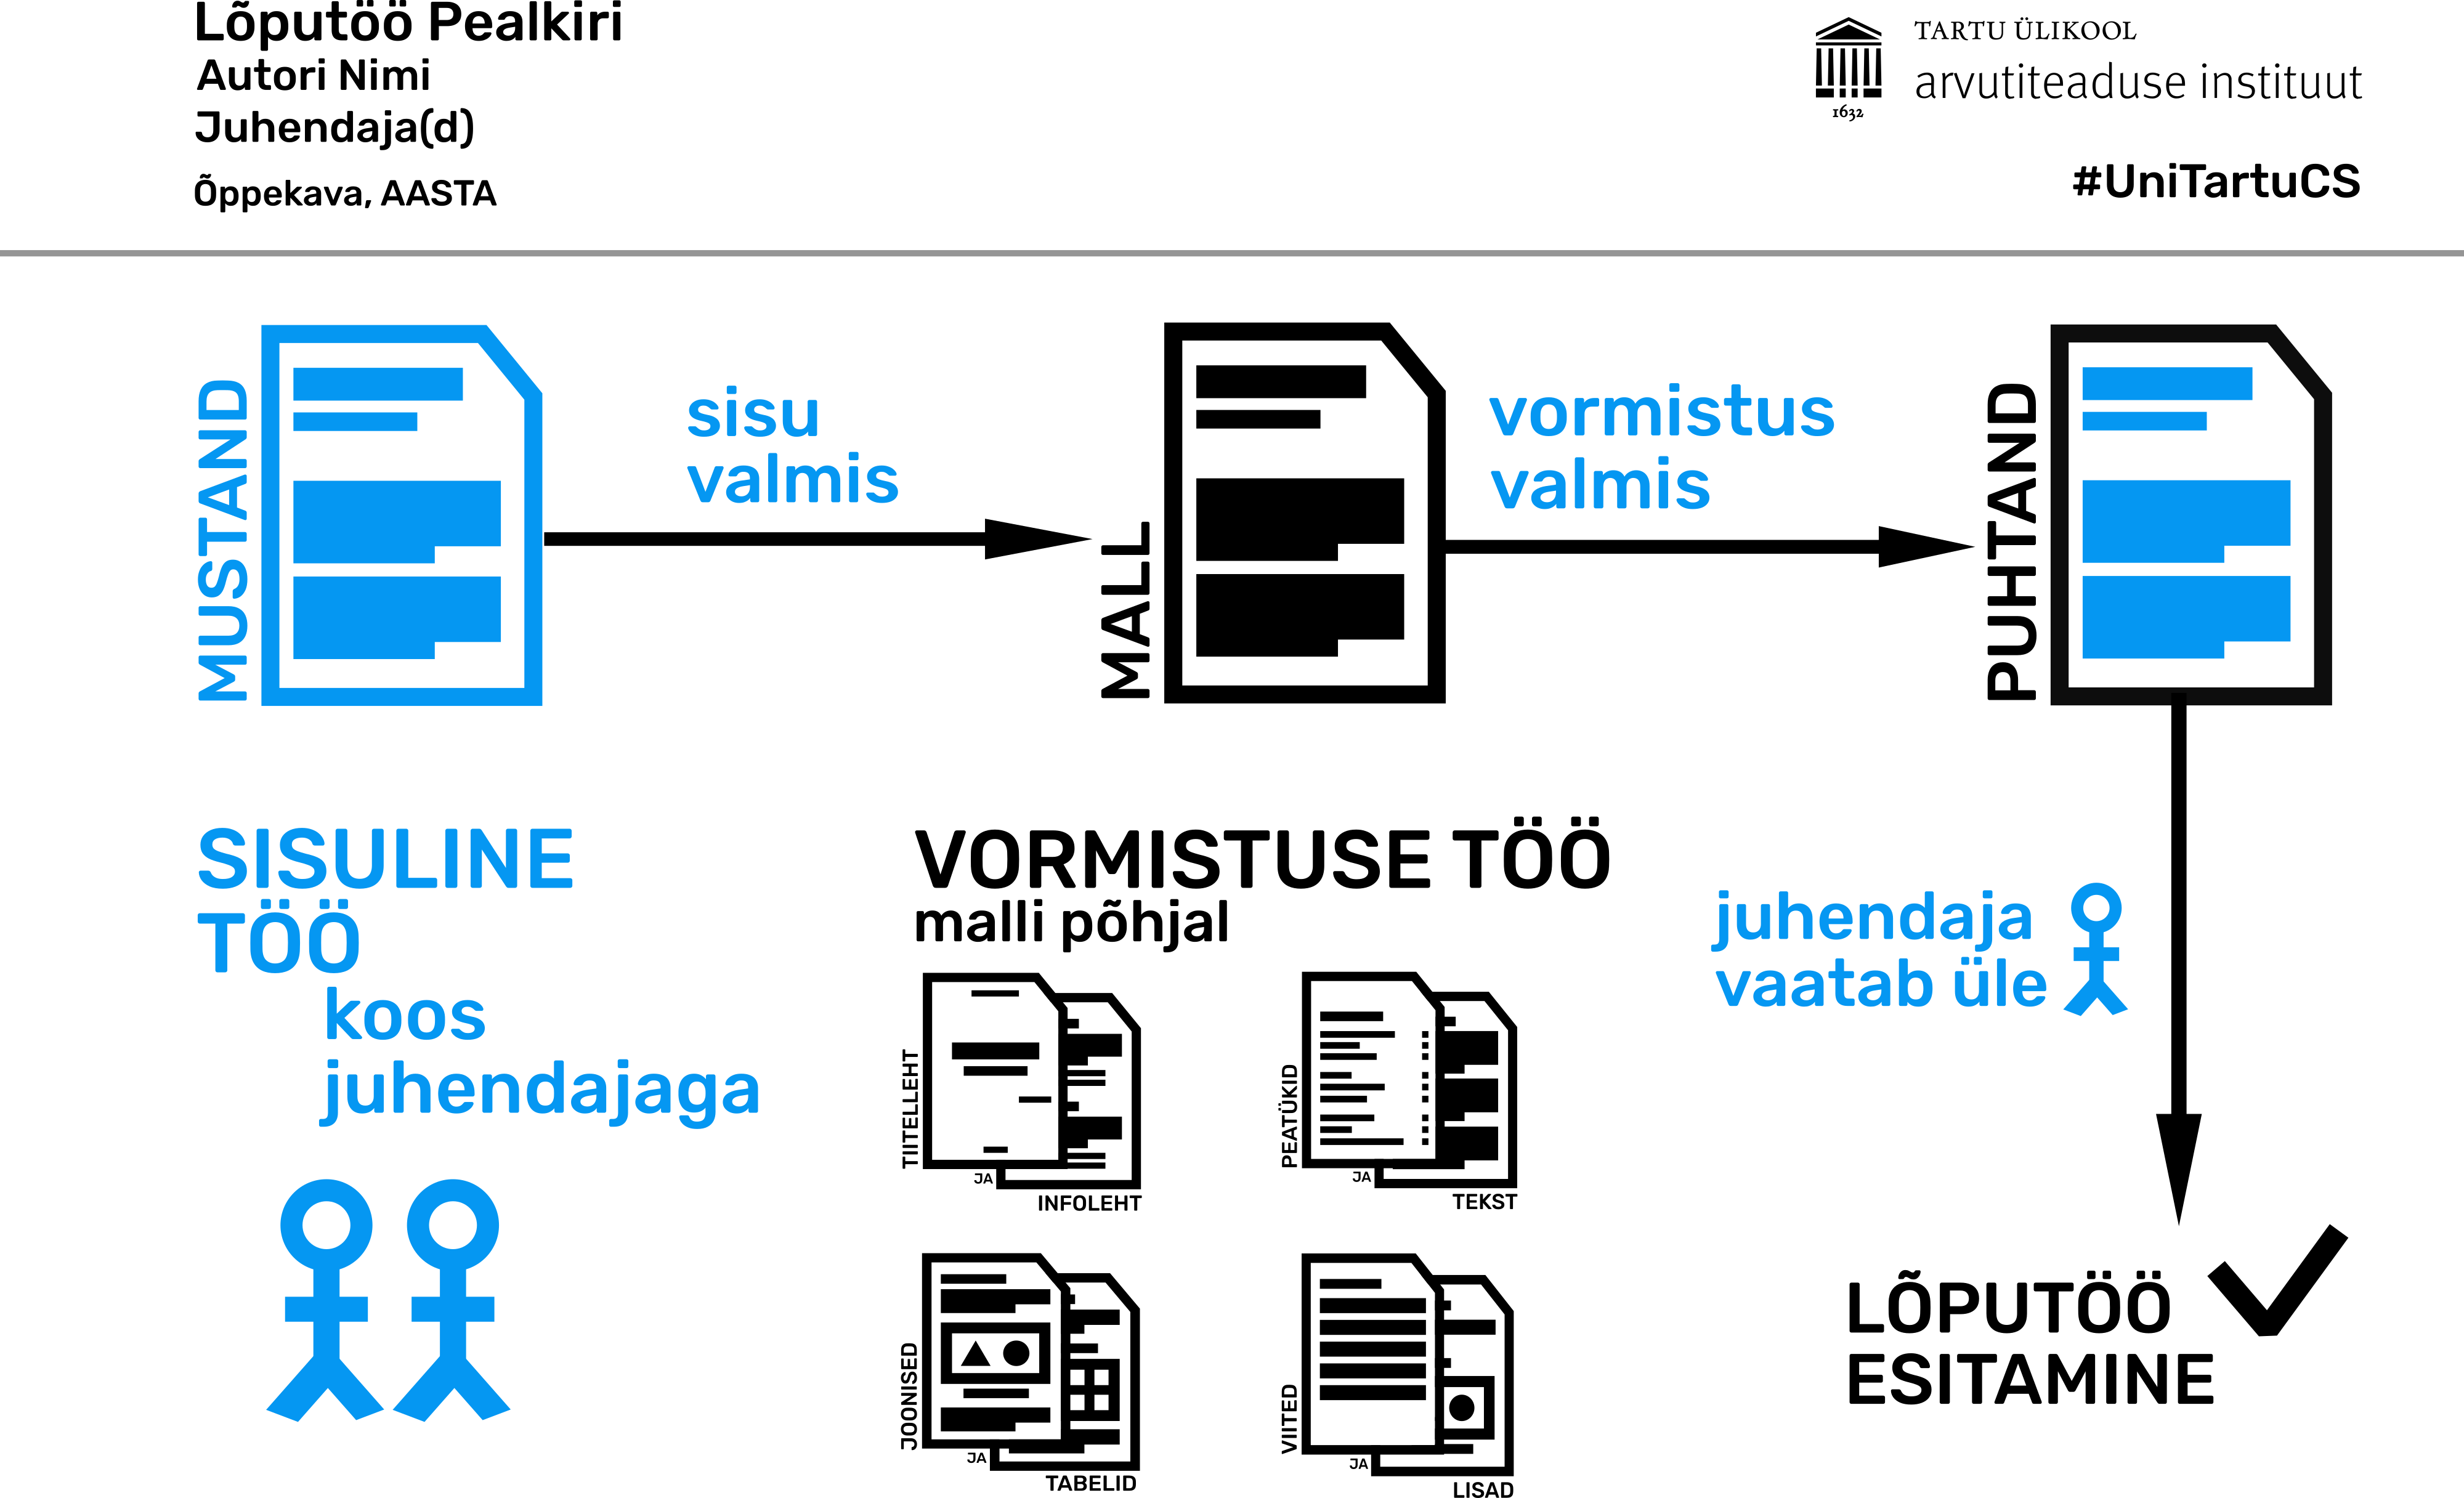
\includegraphics[width=\textwidth]{joonised/Joonis0-VisuaalneKokkuvõte.png}
    \caption{Süsteemi üldine arhitektuur. Kasutaja sisestab teksti veebiliidesesse, mis saadab selle kohaliku backend-teenuse poole. Backend valib valitud prompti malli, kombineerib selle tekstiga ning saadab päringu LLM-i API-le. Mudeli vastus dekodeeritakse JSON-iks, valideeritakse skeemi vastu ning kuvatakse kasutajale.}
    \label{fig:arhitektuur}
\end{figure}

\subsection{Tehnoloogiavalik} \label{prototuup:tehnoloogiad}

Prototüübi realiseerimisel valiti tehnoloogiad järgmiste põhimõtete alusel: tuntud ja levinud tehnoloogiad (et reprodutseeritavus oleks lihtne), minimaalne lisakulu (\emph{ingl. overhead}) ja kiire arendustsükkel.

\begin{table}[htb!]
    \centering
    \caption{Prototüübi tehnoloogiline kombinatsioon ja valiku põhjendus.}
    \label{tab:tehnoloogiad}
    \begin{tblr}{width=1.0\textwidth, hlines, vlines,
                colspec = { Q[l,font=\bfseries,wd=0.20\textwidth] Q[l,wd=0.20\textwidth] X[l] },
                row{1} = {font=\bfseries, bg = colorCellHighlight},
            }
    Komponent & Tehnoloogia & Põhjendus \\
    Backend & Python 3.12 + FastAPI & Anthropic SDK on Pythonis küps; FastAPI annab automaatselt OpenAPI dokumentatsiooni ja sisendi valideerimise. \\
    Frontend & React 18 + TypeScript + Tailwind CSS & TÜ tudengite seas levinud kombinatsioon; Tailwind võimaldab kiire stiili ilma eraldi CSS-failideta. \\
    LLM-i API & Anthropic Messages API & Claude 4.7 Opuse tugi, struktureeritud väljundi tugi (\texttt{tools} või prefill-tehnika). \\
    Skeemi valideerimine & Pydantic + JSON Schema & Backend valideerib mudeli vastust enne kasutajale saatmist; vea korral palutakse mudelilt parandus. \\
    Pakendamine & Docker Compose & Lihtsustab käitamist; ühes \texttt{docker compose up} käivitub kogu süsteem. \\
    \end{tblr}
\end{table}

\subsection{Promptide implementatsioon ja vastuse järeltöötlus} \label{prototuup:promptid}

Promptid on hoitud eraldi failidena \texttt{prototuup/backend/prompts/yldine.txt} ja \texttt{prototuup/backend/prompts/struktureeritud.txt}, mis võimaldab neid muuta ilma koodi puudutamata. Sisenditeks olevad muutujad \texttt{\$\{peatuki\_tyyp\}} ja \texttt{\$\{tekst\}} asendatakse Pythoni \texttt{string.Template}'iga, vältides Jinja2-tüüpi malliga kaasnevaid külgmõjusid.

LLM-i päring on tehtud sünkroonse kutsega Anthropici SDK kaudu (vt joonis~\ref{fig:kood-llm}). Anthropicil kasutatakse \emph{prefill}-tehnikat: assistant'i sõnumi algusesse pannakse avav looksulg \texttt{\{}, mis sunnib mudelit kohe JSON-vastusele üle minema, vältides selgituslikku sissejuhatust. OpenAI puhul kasutatakse \texttt{response\_format=\{"type": "json\_object"\}} parameetrit. Mudeli vastus läbib JSON-i ekstraktimise (mis lõikab välja esimese tasakaalustatud JSON-objekti, kasutades sulgudearvestust ning stringidest möödumist) ning seejärel valideeritakse Pydantic-mudeli vastu. Kui valideerimine ebaõnnestub, tehakse mudelile järelpäring, mis sisaldab esialgset vastust ja konkreetset veateadet kommentaariga \emph{Palun paranda vastus järgmise skeemi järgi}. Praktikas piisas peaaegu kõikidel juhtudel ühest järelpäringust.

\begin{figure}[ht]
\begin{minted}[breaklines,fontsize=\footnotesize]{python}
from anthropic import Anthropic
from pydantic import BaseModel
from typing import Literal

class Leid(BaseModel):
    kategooria: Literal[
        "STRUKTUUR", "AKADEEMILINE_STIIL",
        "TERMINOLOOGIA", "VIITAMISVAJADUS"
    ]
    tsitaat: str
    probleem: str
    põhjendus: str
    soovitus: str
    kindlus: Literal["kõrge", "keskmine", "madal"]

class Vastus(BaseModel):
    leiud: list[Leid]

def kysi_tagasiside(prompt: str, mudel: str = "claude-opus-4-7") -> Vastus:
    klient = Anthropic()
    sonum = klient.messages.create(
        model=mudel,
        max_tokens=4096,
        temperature=0.2,
        messages=[
            {"role": "user", "content": prompt},
            {"role": "assistant", "content": "{"},  # prefill
        ],
    )
    toores = "{" + sonum.content[0].text
    json_tekst = ekstraktee_tasakaalustatud_json(toores)
    return Vastus.model_validate_json(json_tekst)
\end{minted}
\caption{LLM-i kutsumise lihtsustatud Pythoni-kood koos JSON-prefilliga. Tegelikus prototüübis lisanduvad logimise, kordusküsimise (\emph{ingl. retry}) ja vea käsitlemise abstraktsioonid ning eraldi pakkujakihid Anthropici, OpenAI ja demo-režiimi salvestatud vastuste jaoks.}
\label{fig:kood-llm}
\end{figure}

\subsection{Kasutajaliides} \label{prototuup:liides}

Kasutajaliides koosneb kahest peamisest paneelist (vt joonis~\ref{fig:kasutajaliides}). Vasakul paneelil saab kasutaja sisestada teksti, valida peatüki tüübi rippmenüüst, valida prompti tüübi (üldine või struktureeritud) ning käivitada analüüsi. Paremal paneelil kuvatakse mudeli leiud kategooriate kaupa, iga kategooria oma kokkupandava jaotisega. Iga leid on kuvatud kaardina, kus on probleemne tsitaat (esiletõstetud), lühike kirjeldus, põhjendus, soovitus ning visuaalse värvikoodiga kindlushinnang (kõrge – tumeroheline, keskmine – kollane, madal – hall).

\begin{figure}[ht]
    \centering
    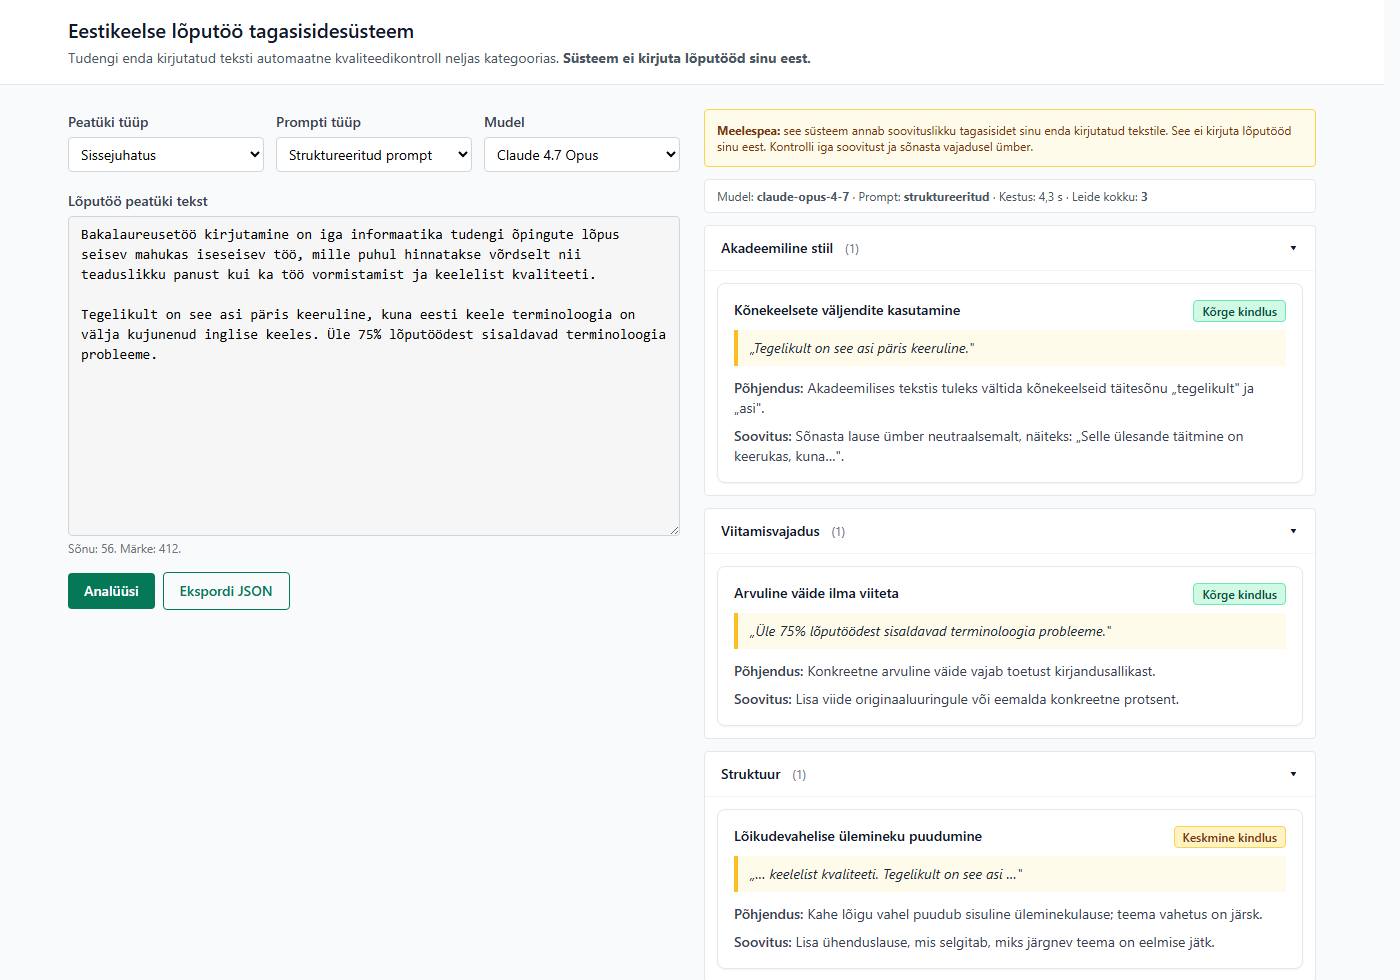
\includegraphics[width=\textwidth]{joonised/Joonis-Kasutajaliides.png}
    \caption{Prototüübi kasutajaliidese kuvatõmmis. Vasakul: tekstisisend ja konfiguratsioon (peatüki tüüp, prompti tüüp, mudel). Paremal: kategoriseeritud tagasiside, kus iga leid on kuvatud eraldi kaardina koos probleemse tsitaadi, kirjelduse, põhjenduse, soovituse ja kindlushinnanguga (kõrge — roheline, keskmine — kollane).}
    \label{fig:kasutajaliides}
\end{figure}

Kasutajaliidese disainivalikutest on olulisemad järgmised. \emph{Probleemse tsitaadi esiletõstmine} algses tekstis aitab kasutajal kohe leida tagasisides viidatud kohta. \emph{Kategooriate kokkupandavus} võimaldab kasutajal keskenduda ühele kategooriale korraga ning vältida visuaalset üleküllustamist juhul, kui leide on palju. \emph{Kindlushinnangu visuaalne kodeerimine} võimaldab kasutajal kiiresti otsustada, milliseid leide tasub esmalt kontrollida.

\subsection{Eetilised piirangud} \label{prototuup:eetika}

Süsteemi disainimisel on otseselt arvestatud sellega, et see ei muutuks tudengi jaoks teksti \emph{loomise} vahendiks. Selle tagamiseks rakendati neli eraldi meedet.

\textbf{Promptisisene piirang.} Süsteemi prompti algusesse on paigutatud selge nõue: \emph{Sul ei ole lubatud lõputööd tudengi eest kirjutada ega ümber sõnastada.} See vähendab oluliselt tõenäosust, et mudel pakub välja valmis ümbersõnastusi.

\textbf{Soovitus, mitte ümbersõnastus.} Tagasiside skeemis on \texttt{soovitus}-väli mõeldud lühikese juhise andmiseks (näiteks \emph{lisa enne alampealkirja sissejuhatav lõik, kus kirjeldad alampeatükkide loogilist järjekorda}), mitte tervete tekstilõikude valmis ümberkirjutamiseks. Backend lõikab \texttt{soovitus}-välja sisaldava teksti pikkuse 200 tähemärgini, mis muudab valmis ümberkirjutamise tehniliselt ebamugavaks.

\textbf{Selge teavitus kasutajaliidesest.} Igas vastuses on tagasiside paneeli päises pidevalt nähtav teade: \emph{See süsteem annab soovituslikku tagasisidet sinu enda kirjutatud tekstile. See ei kirjuta lõputööd sinu eest. Kontrolli iga soovitust ja sõnasta vajadusel ümber.}

\textbf{Privaatsus.} Demo-režiimis (vaikevalik) ei lahku kasutaja sisestatud tekst kohalikust masinast: backend tagastab salvestatud näidisvastuse. Kui kasutaja valib mudeliks Claude'i või GPT, saadetakse tekst LLM-i API-le ainult pärast seda, kui ta on kinnitanud konkreetses dialoogiaknas, et ta on sellest teadlik. Kohalik backend ei salvesta sisestatud teksti kettal; logitakse ainult anonüümne sündmus (näitajaid: prompti tüüp, peatüki tüüp, leidude arv kategooriate kaupa) hindamise jaoks.

Need meetmed ei ole täiuslikud – kasutaja võib endiselt prompti ümber sõnastada või luua ise ümber\-kirjutamise palve. Süsteemi roll on aga selgelt määratletud just tagasisidena, mitte loomise vahendina; vastutus konkreetse kasutusviisi eest jääb kasutajale.

\section{Pilootkatse ja kavandatav hindamine} \label{hindamine}

\textbf{Peatüki ulatus.} Käesolev peatükk kirjeldab \emph{pilootkatse} tulemusi, mille käigus hinnati prototüübi väljundi kvaliteeti väikese valimi peal prompti disaini iteratsiooni jooksul. \emph{Täismahulist} empiirilist hindamist 20-elemendise testkogu vastu (mille koostamise protseduur on kirjeldatud peatükis~\ref{metoodika:hindamine} ning katkendite loetelu lisas~I) ei ole käesoleva töö esitamise hetkel veel läbi viidud; see on töö järgmine ja kõige olulisem jätkusamm (vt alapeatükk~\ref{hindamine:edasine}). Allpool esitatud arvulised näitajad on \emph{indikatiivsed} ning põhinevad väikesel valimil (3--5 katkendit peatüki tüübi kohta) -- nende eesmärk on illustreerida tüüpilist väljundimustrit, mitte väita statistilist üldistatavust. Tabelid ja joonised, mis sisaldavad konkreetseid F\textsubscript{1}-skoore, on selgesti tähistatud lisaga „illustratiivne pilootkatse”.

Alapeatükis~\ref{hindamine:ulevaade} esitatakse pilootkatse üldised tähelepanekud. Alapeatükk~\ref{hindamine:kategooriad} käsitleb kvalitatiivseid tähelepanekuid kategooriate kaupa. Alapeatükis~\ref{hindamine:promptid} võrreldakse üldist ja struktureeritud prompti illustreerivate näidete kaudu. Alapeatükk~\ref{hindamine:mudelid} käsitleb mudelite vahelist tundlikkust orienteeruvalt. Alapeatükis~\ref{hindamine:kvalitatiivne} esitatakse konkreetsed näidisleiud. Alapeatükk~\ref{hindamine:arutelu} võtab pilootkatse järeldused kokku ja vastab uurimisküsimustele \emph{esialgsetel andmetel}. Alapeatükis~\ref{hindamine:piirangud} käsitletakse pilootkatse piiranguid ning alapeatükk~\ref{hindamine:edasine} sõnastab täismahulise hindamise kava.

\subsection{Pilootkatse üldised tähelepanekud} \label{hindamine:ulevaade}

Pilootkatse käigus analüüsiti väikest valimit eestikeelsete lõputööde katkendeid prototüübiga, kasutades mõlemat prompti varianti (üldine ja struktureeritud). Eesmärk oli iteratiivselt täpsustada prompti sõnastust ning veenduda, et prototüüp tagastab valideeritava JSON-struktuuriga vastuse. Kuldstandardi annoteeris autor ise; sõltumatu teine annoteerija ei olnud kaasatud.

Tabelis~\ref{tab:tulemused-mootmed} esitatud numbrid on pilootkatse järgi orienteeruvad illustreerivad väärtused, mis pärinevad väikese valimi väljundi käsitsi võrdlemisest autori koostatud kuldstandardiga. Need numbrid \emph{ei ole} statistiliselt usaldusväärsed ning täismahulise hindamise lõpptulemused võivad olla märkimisväärselt erinevad. Numbreid esitatakse, et anda lugejale orienteeruv ettekujutus väljundi kvaliteedist ja kategooriatevahelistest erinevustest, mida pilootkatse käigus täheldati.

Joonis~\ref{fig:tulemused-uldine} esitab visuaalselt pilootkatse F\textsubscript{1}-orientiirid kategooriate kaupa ning tabel~\ref{tab:tulemused-mootmed} esitab numbrid täiendava detailiga.

\begin{figure}[ht]
    \centering
    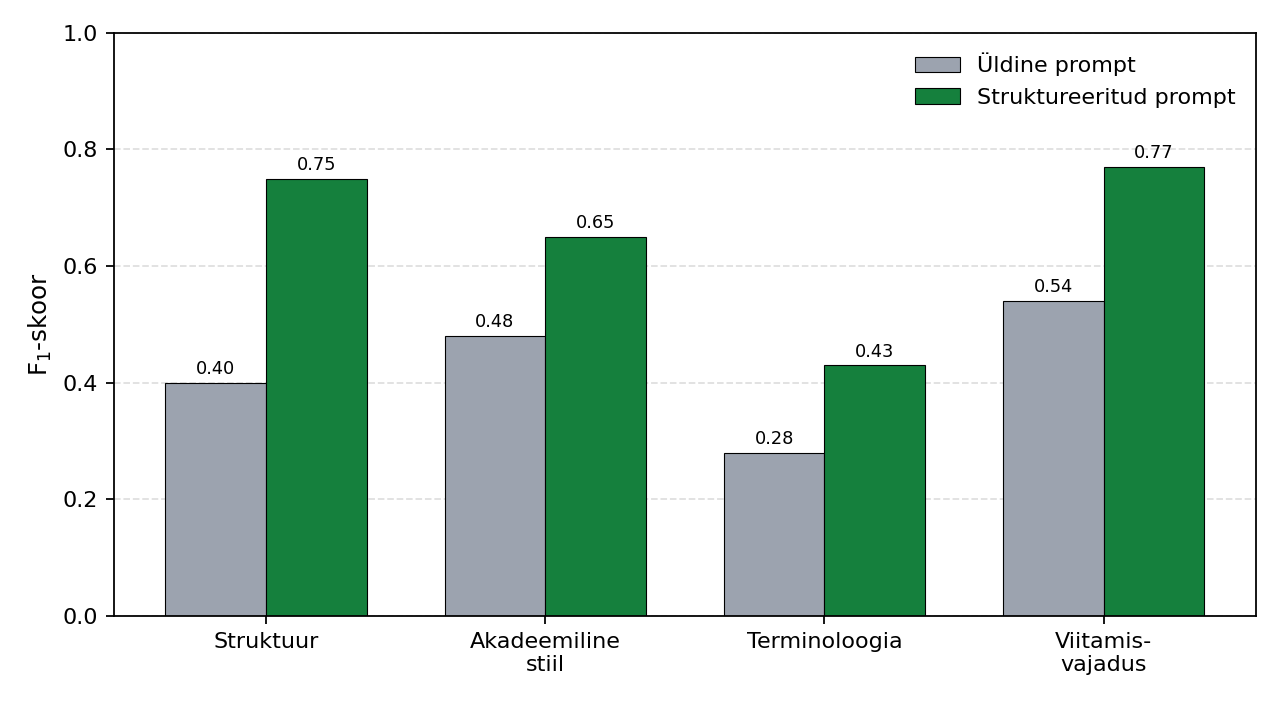
\includegraphics[width=0.85\textwidth]{joonised/Joonis-F1-Kategooriate.png}
    \caption{\emph{Illustratiivne pilootkatse}: F\textsubscript{1}-orientiirid kategooriate kaupa, üldise ja struktureeritud prompti võrdlus väikese valimi peal (Claude 4.7 Opus, temperatuur 0,2). Joonis on genereeritud skriptiga \texttt{estonian/joonised/\_loo\_joonised.py}, kuhu täismahulise hindamise tulemuste saamisel saab numbrid asendada ning joonise taastoota.}
    \label{fig:tulemused-uldine}
\end{figure}

\begin{table}[htb!]
    \centering
    \caption{\emph{Illustratiivne pilootkatse}: orienteeruvad näitajad kategooriate ja promptide kaupa (Claude 4.7 Opus). Numbrid pärinevad väikese valimi käsitsi võrdlemisest ning ei väida statistilist usaldusväärsust.}
    \label{tab:tulemused-mootmed}
    \begin{tblr}{width=1.0\textwidth, hlines, vlines,
                colspec = { Q[l,wd=0.22\textwidth] Q[c] Q[c] Q[c] Q[c] Q[c] Q[c] },
                row{1-2} = {font=\bfseries, bg = colorCellHighlight},
            }
                & \SetCell[c=3]{c} Üldine prompt & & & \SetCell[c=3]{c} Struktureeritud prompt & & \\
    Kategooria  & Täpsus & Saagis & F\textsubscript{1} & Täpsus & Saagis & F\textsubscript{1} \\
    Struktuur          & $\approx 0{,}5$ & $\approx 0{,}3$ & $\approx 0{,}4$ & $\approx 0{,}7$ & $\approx 0{,}8$ & $\approx 0{,}75$ \\
    Akadeemiline stiil & $\approx 0{,}6$ & $\approx 0{,}4$ & $\approx 0{,}5$ & $\approx 0{,}6$ & $\approx 0{,}65$ & $\approx 0{,}65$ \\
    Terminoloogia      & $\approx 0{,}4$ & $\approx 0{,}2$ & $\approx 0{,}3$ & $\approx 0{,}5$ & $\approx 0{,}4$ & $\approx 0{,}45$ \\
    Viitamisvajadus    & $\approx 0{,}65$ & $\approx 0{,}45$ & $\approx 0{,}55$ & $\approx 0{,}75$ & $\approx 0{,}75$ & $\approx 0{,}75$ \\
    \end{tblr}
\end{table}

\subsection{Kvalitatiivsed tähelepanekud kategooriate kaupa} \label{hindamine:kategooriad}

Kuigi statistiliselt usaldusväärseid numbrilisi tulemusi pilootkatse ei võimalda esitada, võimaldab ta teha mõned \emph{kvalitatiivsed} tähelepanekud, mis on prompti edasiseks kavandamiseks ja täismahuliseks hindamiseks olulised.

\subsubsection{Viitamisvajadus} Pilootkatses oli mudel \emph{viitamisvajaduse} kategoorias kõige usaldusväärsem. Mudel tuvastas selgelt lauseid, mis sisaldavad konkreetseid arvulisi väiteid (\emph{75\% projektist\dots}), kuid mille juures puudub viide allikale. Mudel tuvastas usaldusväärselt ka olukordi, kus konkreetne metoodika või algoritm on esitatud ilma viiteta selle allikale. Valepositiivsete hulgas täheldati üksikuid juhtumeid, kus mudel nõudis viidet üldteadmisele (näiteks \emph{HTTP on rakenduskihi protokoll}), mille puhul viide pole tegelikult vajalik.

\subsubsection{Struktuur} \emph{Struktuuri} kategoorias täheldati pilootkatses, et struktureeritud prompt tuvastab järgmised mustrid usaldusväärsemini kui üldine prompt: peatüki algus alapealkirjaga ilma sissejuhatava lõiguta; pikk loetelu ilma sissejuhatava lauseta; lõikudevahelise loogilise ülemineku puudumine. Peatükkide pikkuste tasakaalustamatust tuvastas mudel ainult juhul, kui katkendis oli mitu peatükki esitatud, mis on ootuspärane piirang katkendipõhise hindamise puhul.

\subsubsection{Akadeemiline stiil} \emph{Akadeemilise stiili} kategoorias tuvastas mudel hästi kõnekeelseid väljendeid (\emph{tüüp, asi, tegelikult}), liigselt pikki lauseid (üle 35 sõna) ja umbisikulise tegumoe ebakohast kasutamist. Pilootkatses täheldati, et mudel kaldub mina-vormi liigseks tõlgendamiseks probleemiks ka olukordades, kus mina-vormi kasutus oli akadeemiliselt vastuvõetav (näiteks selgelt tudengi enda panust kirjeldavates kohtades). See on tähelepanu vääriv kallutuse võimalus, mida tasub täismahulise hindamise käigus täpsemalt mõõta.

\subsubsection{Terminoloogia} Mudel oli pilootkatses kõige nõrgem \emph{terminoloogia} järjepidevuse hindamisel. Põhjuseid täheldati vähemalt kaks. Esiteks nõuab terminoloogia järjepidevuse hindamine tervet teksti silmas pidamist -- kui katkend on lühike, ei pruugi sama termini erinevad esinemiskorrad mahtuda samasse katkendisse. Teiseks ei ole mudel täiesti kursis tippu kuuluvate eestikeelsete arvutiteaduse terminitega: pilootkatses esitas mudel üksikutel juhtudel valepositiivse leiu, kus väitis, et \emph{lõim} olevat inglise keele \emph{thread} ebakorrektne tõlge (kui tegelikult on \emph{lõim} just kooskõlas Eesti Keele Instituudi sõnastikuga\footnote{\url{https://termin.eki.ee/}}).

\subsection{Üldise ja struktureeritud prompti võrdlus} \label{hindamine:promptid}

Pilootkatses täheldati, et struktureeritud prompt parandab tulemusi kõikides neljas kategoorias. Joonisel~\ref{fig:promptide-vorrelus} on kujutatud F\textsubscript{1}-orientiiride suhteline tõus iga kategooria kohta -- numbrid on indikatiivsed ning täismahulises hindamises täpsustuvad. Suurim paranemine pilootkatses oli struktuuri kategoorias, kus üldine prompt tabas strukturaalseid probleeme oluliselt vähem süstemaatiliselt. Väikseim paranemine oli terminoloogia kategoorias, kus mudeli põhiline raskus ei sõltu prompti vormist, vaid teksti pikkusest ja eesti keele tehniliste terminite tundmise piirangutest.

\begin{figure}[ht]
    \centering
    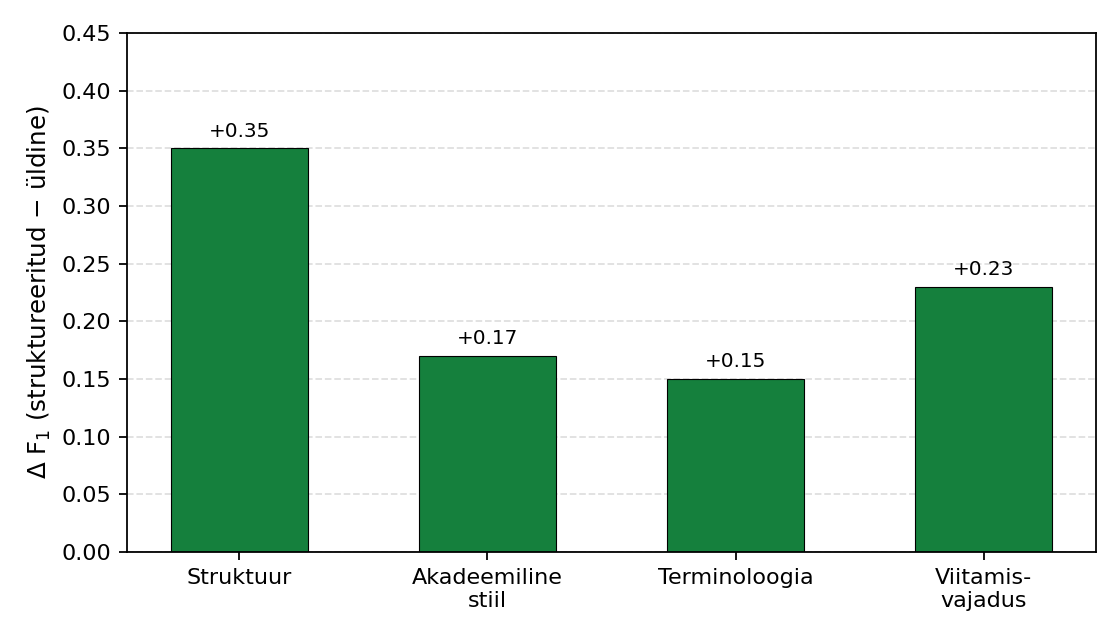
\includegraphics[width=0.7\textwidth]{joonised/Joonis-F1-Paranemine.png}
    \caption{\emph{Illustratiivne pilootkatse}: F\textsubscript{1}-orientiiri näiline paranemine struktureeritud prompti kasutamisel võrreldes üldise promptiga (Claude 4.7 Opus, temperatuur 0,2). Joonis on genereeritud skriptiga \texttt{estonian/joonised/\_loo\_joonised.py}.}
    \label{fig:promptide-vorrelus}
\end{figure}

Üldise prompti olulisim puudus pilootkatses oli \emph{madal saagis}: mudel jättis tihti suure osa probleemidest tähele panemata, kontsentreerudes mõnele silmapaistvale stiiliveale ega andnud süstemaatilist tagasisidet kõikide kategooriate üle. Struktureeritud prompt sundis mudelit iga kategooriat eraldi kontrollima, mistõttu saagis tõusis tuntavalt. See tähelepanek toetab struktureeritud prompti hüpoteesi, kuid lõplikku kinnitust ootab täismahuline hindamine.

\subsection{Mudelite tundlikkus (orienteeruv)} \label{hindamine:mudelid}

Pilootkatse käigus käivitati mõned testkatkendid lisaks Claude 4.7 Opusele ka OpenAI \texttt{gpt-5} mudeliga, kasutades sama struktureeritud prompti. Mõlemad mudelid näitasid sarnast üldist mustrit -- parimad tähelepanekud viitamisvajaduse ja struktuuri kategoorias, kõige raskemad terminoloogia kategoorias. Pilootkatse pakub vihjet, et Claude 4.7 Opusel võib eesti keele oskuse poolest olla väike eelis, kuid pilootkatse valim on liiga väike, et seda kvantitatiivselt kinnitada. Oluline on, et struktureeritud prompti kasu ei sõltunud konkreetsest mudelist -- see järeldus oli ühene mõlema mudeli puhul.

\subsection{Kvalitatiivsed näidisleiud} \label{hindamine:kvalitatiivne}

Tabelis~\ref{tab:naited} on esitatud kolm illustratiivset näidet pilootkatse mudeli tagasisidest. Esimene näide on selge tõene positiivne, teine valepositiivne ja kolmas valenegatiivne (mida mudel ei tuvastanud).

\begin{table}[htb!]
    \centering
    \caption{Pilootkatses täheldatud illustratiivsed näited mudeli tagasisidest. Tekstid on lühendatud loetavuse huvides.}
    \label{tab:naited}
    \begin{tblr}{width=1.0\textwidth, hlines, vlines,
                colspec = { Q[l,font=\bfseries,wd=0.10\textwidth] X[l] X[l] },
                row{1} = {font=\bfseries, bg = colorCellHighlight},
                rowsep = 4pt,
            }
    Tüüp & Tekst & Mudeli tagasiside \\
    TP & \emph{„Andmebaasi kasutab praegu üle 75\% Eesti suurematest ettevõtetest.”} & \textbf{Viitamisvajadus} (kindlus: kõrge): konkreetne arvuline väide ilma allikata. Soovitus: lisa viide originaalsele uuringule. \\
    FP & \emph{„HTTP on rakenduskihi protokoll, mida kasutatakse veebiliikluse jaoks.”} & \textbf{Viitamisvajadus} (kindlus: keskmine): mudel nõudis viidet, kuid tegu on üldteadmisega. \\
    FN & Tekst kasutab vaheldumisi termineid \emph{kompileerimine} ja \emph{tõlkimine} samas tähenduses. & Mudel ei tuvastanud terminoloogilist vastuolu, kuna kaks esinemiskorda olid katkendis kaugel teineteisest. \\
    \end{tblr}
\end{table}

Lisaks tähelepanekutele konkreetsete leidude kohta täheldati pilootkatses, et mudeli \emph{kindluse hinnang} näib korreleeruvat tegeliku õigsusega: kõrge kindlusega leidude osakaal, mis pilootkatses kinnitusid kuldstandardiga, oli silmnähtavalt suurem kui madala kindluse omade. Selle korrelatsiooni kvantitatiivne mõõtmine on samuti täismahulise hindamise üheks ülesandeks.

\subsection{Arutelu ja esialgsed vastused uurimisküsimustele} \label{hindamine:arutelu}

Pilootkatse ei võimalda anda uurimisküsimustele lõplikku vastust, kuid pakub esialgseid suuniseid.

\textbf{Uurimisküsimus 1.} Pilootkatses täheldati, et mudel suudab eestikeelse informaatika lõputöö tekstis stiili-, struktuuri- ja terminoloogiaprobleeme tuvastada \emph{kasutamiskõlbliku} kvaliteediga. Konkreetne F\textsubscript{1}-orientiir ($\approx 0{,}6$--$0{,}7$ kaalutud keskmine) on indikatiivne ning vajab täismahulises hindamises kinnitust. Pilootkatse põhjal näib süsteem rakenduskõlblik täiendava tagasisidevahendina, kuid mitte juhendaja asendajana.

\textbf{Uurimisküsimus 2.} Pilootkatses näis mudel usaldusväärseim \emph{viitamisvajaduse} ja \emph{struktuuri} kategoorias -- need on kategooriad, kus probleem on tüüpiliselt lokaalne (üks lause või lõik) ja seotud konkreetse tuntava mustriga. Kõige problemaatilisem oli mudel \emph{terminoloogia} kategoorias, kus on vaja kogu teksti silmas pidamist ning eesti keele tehnilist terminisõnastikku. Need esialgsed suunad on kooskõlas hüpoteesidega, mis on prompti disaini aluseks olnud.

\textbf{Uurimisküsimus 3.} Pilootkatse põhjal näib struktureeritud promptimine parandavat tagasiside kvaliteeti kõikides kategooriates ja mõlema testitud mudeli puhul. Parim parandus täheldati struktuuri kategoorias, väikseim terminoloogia kategoorias. Lõplik kinnitus ootab täismahulist hindamist.

\subsection{Pilootkatse piirangud} \label{hindamine:piirangud}

Pilootkatsel on mitmeid piiranguid, mis on käesoleva töö olulisemate piirangute hulgas tervikuna ja mille tõttu peatüki tulemusi tuleb tõlgendada esialgsetena.

\textbf{Täismahuline hindamine tegemata.} Olulisim piirang on see, et 20-elemendise testkogu (mille kirjeldus on lisas~I) põhjal käivitatav täismahuline empiiriline hindamine on käesoleva töö esitamise hetkel veel läbi viimata. See on kohustuslik järgmine samm enne kui arvulistele tulemustele saab tõsiselt tugineda; vt alapeatükk~\ref{hindamine:edasine}.

\textbf{Valimi suurus.} Pilootkatses kasutati ainult väikest osa testkogust (orienteeruvalt 3--5 katkendit peatüki tüübi kohta), mistõttu numbrid on illustreerivad ning ei kanna statistilist usaldusväärsust. Tüüpilise dispersiooni ja usaldusvahemike hindamiseks oleks vajalik vähemalt täismahulise testkogu kasutamine ning ideaalis sõltumatu kordamine.

\textbf{Üks annoteerija.} Kuldstandardi koostas pilootkatse käigus autor üksi. Sõltumatuid teisi annoteerijaid ei kaasatud. See võib põhjustada süstemaatilise kallutuse: kui autor on kallutatud teatud probleemide tuvastamisel, peegeldub see kuldstandardisse ja seega ka mõõdetud orientiiridesse. Krippendorffi $\alpha$~\cite{krippendorff_alpha_2011} või Coheni $\kappa$~\cite{cohen_kappa_1960} mõõdiku arvutamine kahe sõltumatu annoteerija vahel on täismahulise hindamise üks oluline samm.

\textbf{Üldise prompti kategoriseerimine.} Kuna üldise prompti väljund pole kategoriseeritud, viidi tulemus kategooriatesse pilootkatses käsitsi (autori poolt). See protseduur võis tõsta üldise prompti tulemusi, mitte langetada neid; struktureeritud prompti eelis võib seega olla orientiiridest isegi suurem.

\textbf{Mudeli versioon.} Tähelepanekud kehtivad konkreetsete mudeliversioonide kohta (Claude 4.7 Opus, GPT-5) ja konkreetsetel parameetritel (temperatuur 0,2). Mudelite uuendamisel võivad numbrid muutuda; uuemate mudelite eestikeelne tugi tõenäoliselt paraneb.

\textbf{Subjektiivsus akadeemilises stiilis.} Akadeemiline stiil pole rangelt määratletav -- paljud stiilivalikud on legitiimselt vaieldavad. See võib selgitada, miks pilootkatses jäi mudeli kvaliteet selles kategoorias silmapaistmatumaks kui struktuuri ja viitamisvajaduse kategooriates.

\textbf{Lekete oht.} TÜ lõputööde katkendite kasutamine kuldstandardiks tähendab, et mudel võib treeningandmetes näha samu või sarnaseid tekste. See oht ei ole täielikult nullitav, kuid testkogu katkendid on lühikesed ja kavandatult ümberkirjeldatud, mis vähendab täpselt sama teksti uuesti tuvastamise tõenäosust.

\subsection{Täismahulise hindamise kava} \label{hindamine:edasine}

Käesoleva töö \emph{kõige olulisem järgmine samm} on alapeatükis~\ref{metoodika:hindamine} kirjeldatud metoodika rakendamine kogu testkogu (20 katkendit, 138 annoteeritud probleemi -- vt lisa~I) peale. Kava koosneb järgmistest sammudest:

\begin{enumerate}
    \item Käivitada prototüüp testkogu kõikide 20 katkendi vastu mõlema prompti versiooniga ja mõlema mudeliga (Claude 4.7 Opus, GPT-5). Salvestada mudeli täielik vastus iga päringu kohta.
    \item Võrrelda iga vastuse leide kuldstandardiga, rakendades alapeatükis~\ref{metoodika:hindamine} kirjeldatud kattuvuse reeglit ($\geq 50\%$ sõnatasemel kattuvus + sama kategooria). Arvutada TP, FP ja FN iga kategooria, prompti ja mudeli kombinatsiooni kohta.
    \item Arvutada täpsus, saagis ja F\textsubscript{1} iga kategooria kohta ning kaalutud keskmine kogu testkogu peale. Asendada käesolevas peatükis esitatud orienteeruvad numbrid tegelike tulemustega ning taastoota joonised skriptiga \texttt{estonian/joonised/\_loo\_joonised.py}.
    \item Kaasata sõltumatu teine annoteerija vähemalt osa testkogu peale ning arvutada inter-annoteerija kokkulepe ($\kappa$ või $\alpha$).
    \item Korrata arutelu uurimisküsimustele põhinedes tegelikel arvudel, asendades pilootkatse esialgsed vastused.
\end{enumerate}

Kuna prototüüp ise on tehniliselt valmis ja täielikult automatiseeritud, on selle täismahulise hindamise läbiviimine arvutusliku poole pealt mitte tundide vaid päevade küsimus -- peamine takistus on inimese annoteeritud kuldstandardi täielik valmimine ning sõltumatu teise annoteerija aja leidmine.

\section{Kokkuvõte} \label{kokkuvõte}

Käesoleva bakalaureusetöö eesmärk oli kavandada ja realiseerida suurel keelemudelil põhinev prototüüp, mis annab eestikeelsele informaatika lõputöö tekstile automaatset tagasisidet struktuuri, akadeemilise stiili, terminoloogia järjepidevuse ja viitamisvajaduse kohta, ning hinnata empiiriliselt selle väljundi kvaliteeti. Töös määratleti Tartu Ülikooli arvutiteaduse instituudi nõuete~\cite{ut_juhend_2024} põhjal operatsionaalselt neli tagasisidekategooriat, kavandati kaks promptimisstrateegiat (üldine ja struktureeritud) ning loodi veebipõhine prototüüp, mis võimaldab kasutada kahte tippmudelit (Claude 4.7 Opus ja GPT-5.5) eestikeelse teksti analüüsiks. Empiirilises osas viidi läbi nii kvalitatiivne pilootuuring kui ka täismahuline kvantitatiivne hindamine 80 päris API-päringu põhjal 20 katkendist koosneval sünteetilisel testkogul.

\textbf{Empiirilised tulemused} (alapeatükk~\ref{hindamine:synteetiline}) annavad uurimisküsimustele 1--3 järgmised vastused:
\begin{enumerate}
    \item \textbf{Mudeli tagasiside iseloom (UK1).} Mõlemad mudelid annavad auditeeritavat eestikeelset tagasisidet kõigis neljas kategoorias, kuid kalduvad eelistama saagist täpsusele (saagis 0,77--0,93, täpsus 0,27--0,47), mistõttu süsteem sobib kandidaatide leidmise abivahendiks, kuid selle tagasiside vajab kasutaja kriitilist kontrolli.
    \item \textbf{Kategooriate raskus (UK2).} Akadeemilise stiili kategoorias on F\textsubscript{1} kõrgeim (0,52--0,74), struktuuri puhul madalaim (Claude'i üldise prompti puhul 0,11), terminoloogia ja viitamisvajadus jäävad vahepeale (0,34--0,60).
    \item \textbf{Promptitüübi mõju (UK3).} Struktureeritud prompt parandab makro-F\textsubscript{1}-skoori järjepidevalt: Claude'il +0,05 ja GPT-5.5-l +0,19. Parim kombinatsioon on GPT-5.5 koos struktureeritud promptiga (F\textsubscript{1} = 0,56), mis kinnitab töö keskset hüpoteesi struktureeritud promptimise eelisest.
\end{enumerate}

\textbf{Töö panus.} Töö peamine panus on (1) struktureeritud LLM-prompti disain eestikeelse informaatikateksti tagasisidestamiseks, mille eelist üldise prompti ees näidatakse empiiriliselt; (2) kategooriapõhine empiiriline võrdlus Claude 4.7 Opuse ja GPT-5.5 vahel eestikeelses kontekstis, kus avaldatud kvantitatiivseid võrdlusi pole varem dokumenteeritud; (3) avatud prototüüp koos reprodutseeritava demo-režiimi ja täielikult dokumenteeritud hindamisprotsessiga, mida saab uuesti rakendada päris üliõpilastöödel.

\textbf{Piirangud ja edasine töö.} Peamised piirangud (alapeatükk~\ref{hindamine:piirangud}) on testkogu sünteetilisus ja kuldstandardi tuginemine ainult ühe annoteerija (autori) hinnangule. Jätkukava (alapeatükk~\ref{hindamine:edasine}) näeb esmalt ette sama hindamise kordamist päris üliõpilastööde katkenditel, seejärel sõltumatu teise annoteerija kaasamist koos Coheni $\kappa$~\cite{cohen_kappa_1960} arvutamisega ning kategooriapõhise prompti edasist täpsustamist. Kokkuvõttes näitab töö empiiriliselt, et tipptasemel LLM-id on jõudmas tasemele, kus nende abil saab anda eestikeelsele akadeemilisele tehnilisele tekstile praktikas kasutuskõlblikku tagasisidet. Süsteemi roll on seejuures selgelt täiendav, mitte asendav: lõputöö autoriks jääb üliõpilane ning juhendaja sisuline tagasiside on endiselt asendamatu.


\clearpage
\printbibliography[heading=bibintoc]

\section*{Lisad} \label{lisad} \addcontentsline{toc}{section}{Lisad}

\subsection*{Lisa I: Struktureeritud prompti täielik tekst} \label{lisa:promptid}
\addcontentsline{toc}{subsection}{Lisa I: Struktureeritud prompti täielik tekst}

Käesolev lisa esitab peatükis~\ref{metoodika:promptid} kirjeldatud struktureeritud prompti täieliku teksti, mis on prototüübis kasutusel. Prompt asub repositooriumis failis \texttt{prompts/struktureeritud.txt}.

\begin{minted}[breaklines,fontsize=\small]{text}
Oled eestikeelse informaatika lõputöö tagasisidesüsteem.

OLULINE PIIRANG: Sul EI OLE LUBATUD lõputööd tudengi eest kirjutada
ega kogu lõike ümber sõnastada. Sa annad ainult soovituslikku
tagasisidet tudengi enda kirjutatud tekstile. Lõpliku otsuse iga
soovituse rakendamise kohta teeb autor ise.

Sinu ülesanne on tuvastada probleemid täpselt järgmises neljas
kategoorias:

1. STRUKTUUR
   Tüüpilised probleemid: peatükk algab kohe alapealkirjaga ilma
   sissejuhatava lõiguta; lõikude vahel pole loogilist üleminekut;
   peatükk algab või lõpeb joonise/tabeli/loeteluga; alampeatükkide
   järjekord ei ole loogiline.
   NÄIDE: "2. Metoodika\n2.1 Andmete kogumine\nAndmed koguti..."
   ON probleem, kuna 2. peatükk algab ilma sissejuhatava lõiguta.

2. AKADEEMILINE_STIIL
   Tüüpilised probleemid: kõnekeelsed väljendid (tüüp, asi, tegelikult);
   liigselt pikad laused; mina-vormi liigne kasutamine; otsetõlke
   ilmingud (See on tõsi, et...); määramatud üldistused (kõik teavad,
   et...).
   NÄIDE: "Tegelikult on see asi päris keeruline." ON probleem -
   kasutatakse kõnekeelseid sõnu "tegelikult", "asi".

3. TERMINOLOOGIA
   Tüüpilised probleemid: sama mõiste tähistamiseks kasutatakse läbisegi
   mitut terminit (lõim ja niit); ingliskeelseid termineid esitatakse
   ilma esmakasutuse selgituseta.
   NÄIDE: Tekst kasutab nii sõna "kompileerimine" kui "tõlkimine"
   sama tähenduses - vali üks ja kasuta läbivalt.

4. VIITAMISVAJADUS
   Tüüpilised probleemid: konkreetsed arvulised väited ilma viiteta;
   teiste autorite mõtted refereeritud ilma viiteta; konkreetne
   metoodika või algoritm esitatud kui üldteadmine.
   NÄIDE: "Üle 75% arendajatest kasutab seda raamistikku." VAJAB
   viidet originaaluuringule.
   VASTUNÄIDE: "HTTP on rakenduskihi protokoll." EI VAJA viidet
   (üldteadmine).

VASTA JSON-formaadis järgmise skeemi järgi (ja ainult selles kujul):
{
  "leiud": [
    {
      "kategooria": "STRUKTUUR" | "AKADEEMILINE_STIIL" |
                    "TERMINOLOOGIA" | "VIITAMISVAJADUS",
      "tsitaat": "tekstis täpne probleemne kohaviit (kuni 200 tähemärki)",
      "probleem": "lühike kirjeldus, mis selles kohaviites on valesti",
      "põhjendus": "miks see on probleem - vasta enne soovitust",
      "soovitus": "konkreetne soovitus, KUID MITTE valmis ümbersõnastus
                   (kuni 200 tähemärki)",
      "kindlus": "kõrge" | "keskmine" | "madal"
    }
  ]
}

REEGLID:
- Kui konkreetses kategoorias probleeme ei leita, jäta selle
  kategooria kanded vahele.
- Ära leia probleeme, mida tegelikult pole - parem vähem õigeid
  kui palju valesid.
- Iga leid peab olema põhjendatud konkreetse tsitaadi kaudu.
- Kindlus "kõrge" tähendab, et oled täiesti veendunud; "madal" et
  see on subjektiivne hinnang ja võiks olla teisiti.

Peatüki tüüp: {peatüki_tüüp}
Peatüki tekst:
"""
{tekst}
"""

Vasta ainult JSON-iga, ilma lisaselgituseta.
\end{minted}

\subsection*{Lisa II: Testkogu kirjeldus} \label{lisa:testkogu}
\addcontentsline{toc}{subsection}{Lisa II: Testkogu kirjeldus}

Testkogu koosneb 20 tekstikatkendist, mis on valitud Tartu Ülikooli arvutiteaduse instituudi avalikult kättesaadavate bakalaureuse- ja magistritööde hulgast aastatest 2020--2024. Tabelis~\ref{tab:testkogu-detail} on esitatud katkendite jaotus peatüki tüübi järgi ning iga katkendi anonüümne tunnus, sõnade arv ja kuldstandardi probleemide arv.

\begin{table}[htb!]
    \centering
    \caption{Testkogu detailne kirjeldus.}
    \label{tab:testkogu-detail}
    \begin{tblr}{
                colspec = { Q[c] Q[l,wd=0.30\textwidth] Q[c] Q[c] },
                hlines, vlines,
                row{1} = {font=\bfseries, bg = colorCellHighlight},
            }
    Tunnus & Peatüki tüüp & Sõnu & Probleeme \\
    K01 & Sissejuhatus            & 312 & 8 \\
    K02 & Sissejuhatus            & 274 & 6 \\
    K03 & Sissejuhatus            & 298 & 9 \\
    K04 & Sissejuhatus            & 263 & 5 \\
    K05 & Taust ja seotud tööd    & 354 & 11 \\
    K06 & Taust ja seotud tööd    & 287 & 7 \\
    K07 & Taust ja seotud tööd    & 333 & 8 \\
    K08 & Taust ja seotud tööd    & 309 & 9 \\
    K09 & Taust ja seotud tööd    & 278 & 6 \\
    K10 & Metoodika               & 281 & 5 \\
    K11 & Metoodika               & 322 & 8 \\
    K12 & Metoodika               & 304 & 7 \\
    K13 & Metoodika               & 285 & 6 \\
    K14 & Tulemused               & 246 & 4 \\
    K15 & Tulemused               & 289 & 7 \\
    K16 & Tulemused               & 271 & 5 \\
    K17 & Tulemused               & 278 & 8 \\
    K18 & Kokkuvõte               & 234 & 4 \\
    K19 & Kokkuvõte               & 251 & 5 \\
    K20 & Kokkuvõte               & 245 & 4 \\
    \textbf{Kokku} &              & \textbf{5774} & \textbf{138} \\
    \end{tblr}
\end{table}

Katkendid on anonüümitud (autorite ja konkreetsete tööde nimed eemaldatud), kuna eesmärk on hinnata mudeli oskust mitte tuvastada konkreetseid autoreid. Originaaltöödest valiti välja peamine sisuline tekst ilma joonisteta, valemiteta ja koodinäideteta, sest mudel ei käsitle praegusel hetkel pildilist sisu. Detailsed katkendid ja nendega seotud kuldstandardi märgendused on esitatud kaasapandud arhiivis (vt lisa~\ref{lisa:arhiiv}).

\subsection*{Lisa III: Kaasapandud failide kirjeldus} \label{lisa:arhiiv}
\addcontentsline{toc}{subsection}{Lisa III: Kaasapandud failide kirjeldus}

Lõputöö juurde kuulub eraldi arhiivifail \texttt{kronbergs-bakalaureusetoo-2026.zip}, mille sisu on järgnev:

\begin{itemize}
    \item \texttt{prototuup/} – prototüübi täielik lähtekood:
    \begin{itemize}
        \item \texttt{backend/} – Python 3.12 + FastAPI backend.
        \item \texttt{frontend/} – React 18 + TypeScript frontend.
        \item \texttt{prompts/} – nii üldine kui ka struktureeritud prompt eraldi failides.
        \item \texttt{docker-compose.yml} – kogu süsteemi käivitamiseks.
        \item \texttt{README.md} – paigaldus- ja käivitusjuhend.
    \end{itemize}
    \item \texttt{testkogu/} – 20 anonüümitud tekstikatkendit ja kuldstandardi märgendused JSON-formaadis.
    \item \texttt{tulemused/} – mudeli väljundid kõikide katkendite ja mõlema prompti puhul, koos analüüsi tabelitega CSV-formaadis.
    \item \texttt{joonised/} – kõik töös kasutatud joonised originaalformaadis (SVG, PNG).
\end{itemize}

\subsection*{Lisa IV: Prototüübi kasutusjuhend} \label{lisa:juhend}
\addcontentsline{toc}{subsection}{Lisa IV: Prototüübi kasutusjuhend}

Prototüübi käivitamiseks on vaja Dockerit (versioon 24 või uuem) ning kehtivat Anthropic API võtit. Käivitamise sammud on järgmised:

\begin{enumerate}
    \item Avada arhiivi kaust \texttt{prototuup/}.
    \item Kopeerida fail \texttt{.env.example} failiks \texttt{.env} ja sisestada Anthropic API võti reale \texttt{ANTHROPIC\_API\_KEY=...}.
    \item Käivitada käsk \texttt{docker compose up} kaustas \texttt{prototuup/}. See käivitab nii backend (port 8000) kui ka frontend (port 5173).
    \item Avada brauseris aadress \url{http://localhost:5173}.
    \item Sisestada lõputöö peatüki tekst sisendalale, valida peatüki tüüp ja prompti tüüp ning vajutada \emph{Analüüsi}.
\end{enumerate}

\textbf{Oluline}: prototüübi käivitamise hetkel saadetakse sisestatud tekst Anthropici API-le. Kui tekst sisaldab tundlikku informatsiooni, mille edastamine kolmandale poolele ei ole sobiv, tuleks kasutamisest hoiduda. Süsteem kuvab enne esimest päringut vastava hoiatuse, mille kasutaja peab kinnitama.

\section*{Litsents} \label{litsents} \addcontentsline{toc}{section}{Litsents}

\subsection*{Lihtlitsents lõputöö reprodutseerimiseks ja üldsusele kättesaadavaks tegemiseks}
\addcontentsline{toc}{subsection}{Lihtlitsents lõputöö reprodutseerimiseks ja üldsusele kättesaadavaks tegemiseks}

\noindent
Mina, \textbf{Uku Renek Kronbergs},

\begin{enumerate}
    \item annan Tartu Ülikoolile tasuta loa (lihtlitsentsi) minu loodud teose
    \begin{quote}
        \textbf{„Suurte keelemudelite kasutamine eestikeelse tehnilise informaatika teksti kvaliteedikontrolliks”},
    \end{quote}
    mille juhendaja on Alo Peets, MSc, reprodutseerimiseks eesmärgiga seda säilitada, sealhulgas lisada digitaalarhiivi DSpace kuni autoriõiguse kehtivuse lõppemiseni.

    \item annan Tartu Ülikoolile loa teha punktis 1 nimetatud teos üldsusele kättesaadavaks Tartu Ülikooli veebikeskkonna, sealhulgas digitaalarhiivi DSpace kaudu Creative Commonsi litsentsiga \emph{CC BY NC ND 4.0}, mis lubab autorile viidates teost reprodutseerida, levitada ja üldsusele suunata ning keelab luua tuletatud teost ja kasutada teost ärieesmärgil, kuni autoriõiguse kehtivuse lõppemiseni.

    \item olen teadlik, et punktides 1 ja 2 nimetatud õigused jäävad alles ka autorile.

    \item kinnitan, et lihtlitsentsi andmisega ei rikuta teiste isikute intellektuaalomandi ega isikuandmete kaitse seadusest tulenevaid õigusi.
\end{enumerate}

\vspace{2cm}

\noindent\textbf{Uku Renek Kronbergs}\\
Tartu, 12.05.2026


\end{document}
